\chapter{策略的价值与优化}
\label{chap:decision-theory-and-dynamic-risk}
\label{chap:policy-value-and-optimization}

把室温调到目标附近，并没有唯一确定怎样加热。快速升温需要较大的输入，缓慢升温则让
人在较长时间内承受温度偏差；有随机扰动时，两项平均成本接近的策略还可能产生不同的
严重后果。第~\ref{chap:control-theory}章已经讨论策略能否实现目标、使误差收敛并保持
安全，本章进一步问：怎样给这些策略的后果计价，怎样算出给定策略的价值，又怎样选择
成本更低的策略？

评价的对象是策略诱导的状态与行动轨迹。确定性模型中，初态和策略可以确定一条轨迹；
随机模型中，它们通常只确定轨迹的分布。因此，要分清一次执行付出的成本、同一策略
多次执行的平均成本，以及对坏尾部的评价。先确定对象和评价准则，才能计算价值；
计算时固定行动规则，优化时才允许改变规则。这个区别也决定了递推中该对行动概率求和，
还是在可选行动中取最小值。

本章以成本最小化为主要约定。若任务使用收益，只需把收益定义为成本的负值，并将
最小化与最大化成套转换。路线选择保留一个可以逐项枚举的轨迹分布，温度模型连接前章
的反馈设计；信息获取和探索例子则说明行动不仅改变物理状态，也会改变以后知道什么。
这些例子最终都要回答同一个问题：在给定信息、模型和评价口径下，哪项可实施策略更合适？

\section{策略的表示与价值}
\label{sec:policy-representation-and-value}

\subsection{策略的行动与信息}
\label{sec:policy-actions-and-information}

加热器每次收到的是一个输入值，控制器需要规定的却是整套选择规则：温度偏低时怎样选，
下一次读数改变后又怎样选。策略（policy）就是按当时已经知道的信息持续选择行动的规则。
它与一条已经执行的行动序列不同；同一策略遇到不同观测，可以产生不同序列。

先用离散时间和有限状态说明信息次序。状态记为$S_t\in\mathcal S$，行动记为
$A_t\in\mathcal A(S_t)$，每个$\mathcal A(s)$均非空。在行动$A_t$发生之前，完整
状态历史为
\[
  H_t=(S_0,A_0,S_1,\ldots,A_{t-1},S_t).
\]
历史依赖随机策略用概率$\pi_t(a\mid h_t)$指定下一行动，满足
$\pi_t(a\mid h_t)\geq0$及$\sum_a\pi_t(a\mid h_t)=1$，并仅支持当前允许行动。
确定性策略将全部质量放在某个行动上。连续行动时使用可测概率核
$\pi_t(\mathrm da\mid h_t)$，而不是对单个实数行动指定密度而忘记可能的原子质量。
策略的随机数在使用时产生，不得包含未来环境噪声的信息。

若策略只读取当前状态，写作$\pi_t(a\mid s)$，称为Markov策略；若规则还不随时间
改变，写作$\pi(a\mid s)$，称为平稳Markov策略。只去掉历史依赖不等于去掉时间依赖：
距离截止时间还有多久，常会改变合理的动作。前章的开环序列、状态反馈和输出反馈，
分别规定了这些规则怎样接入实际系统，见定义
~\ref{def:control-open-loop-state-output-feedback}。

若只能观察$Y_t$，允许信息是
$\mathcal I_t=\sigma(Y_0,A_0,\ldots,A_{t-1},Y_t)$，策略不能直接读取$S_t$。
即使观测与状态同维，也不能把带噪声读数当作真实状态。
第~\ref{chap:dynamical-systems-and-state-estimation}章状态推断给出的条件分布
$b_t(\mathrm ds)=\mathbb P(S_t\in\mathrm ds\mid\mathcal I_t)$汇集了观测历史对当前
状态的认识。在模型已知、该分布连同时间足以预测后续观测和成本时，可以用$b_t$作为
决策的状态；这不是说一次观测$Y_t$本身满足同样条件。

共同温度模型仍为
\begin{equation}
  x_{t+1}=0.8x_t+u_t+w_{t+1},
  \qquad y_t=x_t+v_t.
  \label{eq:policy-temperature-model}
\end{equation}
$x_t$是相对于环境温度的温差，$u_t$是加热量。本章先取
$w_{t+1}=v_t=0$，默认$u_t\in\mathbb R$，不暗加输入限制。目标$r=2$需要平衡输入
$u^r=2-0.8\times2=0.4$。前章的示例状态反馈
\begin{equation}
  u_t=0.4-0.3(x_t-2)
  \label{eq:policy-temperature-feedback}
\end{equation}
使误差$e_t=x_t-2$满足$e_{t+1}=0.5e_t$。这说明无噪声时误差收敛，却还没有给出
这项策略的成本。若恢复观测噪声，式中的$x_t$须可见，或另行设计基于估计的策略；
直接把$y_t$代入得到的是另一项策略。

\subsection{策略诱导的轨迹}
\label{sec:policy-induced-trajectories}

只有策略还不能预测结果：同一“走捷径”的规则，在不同路况模型下产生的终点概率不同。
因此需要把初态、行动选择和环境转移连接起来。取有限时域$t=0,\ldots,H$，
初始分布为$\mu_0$，阶段成本为$c_t(s,a)$，终端成本为$c_H(s)$。
在每段末状态为$s$的历史$h_t$下，要求受控转移满足
\[
  \mathbb P(S_{t+1}=s'\mid H_t=h_t,A_t=a)=P_t(s'\mid s,a).
\]
这个Markov条件说的是给定当前状态和行动后，过去不再提供预测下一状态的额外信息；
成本也已按同样的状态和行动表示。

\begin{definition}[有限Markov决策过程与策略]
\label{def:decision-finite-mdp-policy}
有限状态集$\mathcal S$、各状态的非空有限行动集$\mathcal A(s)$、初始分布$\mu_0$、
受控转移概率$P_t$、阶段成本$c_t$和终端成本$c_H$组成有限时域
\term{Markov决策过程}（Markov decision process, MDP）。
允许策略可以根据全部已有历史随机选择行动$\pi_t(a\mid H_t)$；
只依赖当前状态时为Markov策略，确定选择时记作$a=\pi_t(s)$。
\end{definition}

这里$S_t,A_t$分别承担前章状态和输入的角色，有限MDP是便于求和计算的版本；
温度模型的连续状态不属于有限集合。若真实转移或成本还依赖未记录的过去，
必须补充状态信息，不能只靠给观测改名来获得Markov性质\scite{math-puterman1994mdp}

现在固定策略$\pi$。对一条状态与行动轨迹
$\tau=(s_0,a_0,s_1,\ldots,a_{H-1},s_H)$，链式法则给出
\begin{equation}
  \mathbb P^\pi(\tau)
  =\mu_0(s_0)\prod_{t=0}^{H-1}
    \pi_t(a_t\mid h_t)P_t(s_{t+1}\mid s_t,a_t).
  \label{eq:policy-trajectory-probability}
\end{equation}
每个因子都对应实际生成的一步：先抽初态，再按当前历史选行动，再由环境生成下一状态。
连续状态时用概率核的逐次积分表达同一构造。输出反馈还要插入观测核，并让行动核仅依赖
已经产生的观测历史；边缘化看不见的状态后，才得到控制器所见的数据分布。

沿用两阶段路线任务。起点$s_0$选择“稳妥”会确定到达终端损失$2$的状态；
选择“捷径”以概率$0.8$到达损失$0$的状态，以概率$0.2$到达损失$6$的状态。
起点行动的阶段成本为零。这里两个阶段指起点选择和终点结算，即$H=1$；
终点没有第二次选择。若策略以概率$p$选择捷径，三条轨迹的概率分别为
\[
  1-p,\qquad 0.8p,\qquad 0.2p.
\]
例如$p=1/2$时为$(0.5,0.4,0.1)$。改变$p$改变行动和终点的联合分布，
但没有改变给定行动后的路况概率。策略随机化与环境随机性因此是两个不同来源。

\subsection{轨迹收益与策略价值}
\label{sec:policy-trajectory-return}

轨迹生成后，可以给实际经过的状态和行动逐项计价。令阶段收益
$r_t(s,a)=-c_t(s,a)$、终端收益$r_H(s)=-c_H(s)$。一条实现轨迹的累计成本和收益为
\begin{equation}
  L(\tau)=\sum_{t=0}^{H-1}c_t(s_t,a_t)+c_H(s_H),
  \qquad G(\tau)=-L(\tau).
  \label{eq:policy-trajectory-cost-return}
\end{equation}
二者是轨迹上的数值，不是策略的平均表现。期望准则下，策略成本为
$J^\pi=\mathbb E^\pi[L]$，策略收益为$\mathbb E^\pi[G]=-J^\pi$；
有限空间可用式~\eqref{eq:policy-trajectory-probability}逐条求和。
后文把成本方向的继续价值记为$V$，因此$V$越小越好。

运行到中途，已经支付的成本不再改变，但后续行动仍可比较。对一段末状态为$s$的历史
$h_t$，一般历史策略的继续成本定义为
\begin{equation}
  J_t^\pi(h_t)=
  \mathbb E^\pi_{h_t}
  \left[\sum_{k=t}^{H-1}c_k(S_k,A_k)+c_H(S_H)\right].
  \label{eq:decision-finite-policy-value}
\end{equation}
下标$h_t$表示固定已知历史，再用策略和转移核重新生成后续过程。
即使该历史在某个初始分布下概率为零，也可以通过这些核定义继续过程，
不必对零概率事件直接作比值条件化。Markov策略下，继续过程只依赖时间与末状态，
于是记作$V_t^\pi(s)$；一般历史策略可能在同一状态记住不同经历，不能无条件这样缩写。
过去累计成本加上$J_t^\pi(h_t)$，才是该历史下整条轨迹总成本的条件期望。

无限时域中，若阶段成本时不变且$|c(s,a)|\leq C$，取$0\leq\gamma<1$，定义
\begin{equation}
  V^\pi(s)=
  \mathbb E_s^\pi\left[\sum_{t=0}^{\infty}\gamma^t c(S_t,A_t)\right].
  \label{eq:decision-discounted-value}
\end{equation}
这里$\pi$仍可依赖全部历史，$s$指定起点。几何级数给出
$|V^\pi(s)|\leq C/(1-\gamma)$，保证累计和与期望有意义。
连续状态的二次成本通常无界，需要另证可积性或矩界；不能只因写了折扣就套用该上界。
无折扣的无限累计也可能发散，尤其是系统持续支付维持目标所需的能耗时。

为共同温度模型定义具体成本，取教学权重$\lambda=1$：
\begin{equation}
  c(x,u)=(x-2)^2+\lambda u^2,\qquad c_H(x)=(x-2)^2.
  \label{eq:policy-temperature-cost}
\end{equation}
第一项惩罚舒适偏差，第二项是按加热幅值平方计价的能耗代理，不声称等于未经标定的
实际电费。这里计的是总输入$u$，不是偏移输入$u-0.4$；两种计价会产生不同的最优策略。
阶段收益始终是$-c(x,u)$。从$x_0=0$执行
式~\eqref{eq:policy-temperature-feedback}两次得到
$(u_0,u_1)=(1,0.7)$和$(x_1,x_2)=(1,1.5)$，
这给出了可逐项评价的一条轨迹。固定规则的计算将在
第~\ref{sec:policy-finite-evaluation}节完成，届时才与其他规则比较。

只有一次行动时，$L$退化为损失$\ell(a,Y)$，收益为$-\ell(a,Y)$。
例如同一阳性概率$0.3$，在对称分类损失与高漏诊损失下会对应不同的行动。
概率只描述结果的可能性，还没有包括后果的代价，更不是多步任务中已经累计未来后果的
继续价值。条件风险和Bayes行动的正式求解留在
第~\ref{sec:decision-bayes-rules}节；先固定策略，下一节比较如何汇总它产生的随机成本。

\section{策略的轨迹价值与风险}
\label{sec:decision-risk-criteria-robustness}

\subsection{平均收益与价值波动}

路线策略已经确定，仍有不止一种评价它的办法。固定走稳妥路线的期望损失为$2$；
固定走捷径的期望损失为$0.8\times0+0.2\times6=1.2$。后者的平均收益较高，
却有$20\%$的概率付出损失$6$。比较策略以前，需要明确任务在意平均成本，还是不能
承受某些严重后果。本节先不改变策略，只比较这些评价口径。

设随机轨迹损失$L$可积。期望$\mathbb E[L]$按发生概率线性汇总所有后果；
对应的期望收益为$-\mathbb E[L]$。为了看清均值遗漏的信息，再考虑两个教学方案
\[
  L_{\mathrm{safe}}=1,\qquad
  L_{\mathrm{tail}}=
  \begin{cases}
    0,&\text{概率 }0.95,\\
    20,&\text{概率 }0.05.
  \end{cases}
\]
二者的期望均为$1$，但第二个方案把全部平均损失集中在最差$5\%$的结果中。
这可以理解为两项已经固定的策略所诱导的终端损失，不能用“平均相同”代替“后果相同”。

有二阶矩时，方差$\operatorname{Var}(L)$衡量围绕均值的二次波动。
均值--方差准则为
\[
  \mathbb E[L]+\lambda\operatorname{Var}(L),\qquad \lambda\geq0.
\]
其中$\lambda$表达波动的权重，与温度成本中的输入权重并无必然关系。该准则同时惩罚
高于和低于均值的偏离，意外变好也会增加方差。更重要的是，它未必尊重逐场景的损失
大小：令$L_1$等概率取$0,2$，令$L_2=2$，则$L_1\leq L_2$，但$\lambda>1$时
\[
  \mathbb E[L_1]+\lambda\operatorname{Var}(L_1)=1+\lambda>2
  =\mathbb E[L_2]+\lambda\operatorname{Var}(L_2).
\]
因此，“厌恶波动”和“避免坏尾部”不是同一个要求。

\begin{definition}[相干风险]
\label{def:decision-coherent-risk}
设风险泛函$\rho:L^1(P)\to\mathbb R$按损失越小越好的方向评价。单调性要求
$L\leq L'$几乎处处时$\rho(L)\leq\rho(L')$；平移等变性要求
$\rho(L+m)=\rho(L)+m$，其中$m$为确定常数。凸性要求
\[
  \rho(\tau L+(1-\tau)L')
  \leq\tau\rho(L)+(1-\tau)\rho(L'),\qquad 0\leq\tau\leq1.
\]
若具有单调性、平移等变性、正齐次性
$\rho(\lambda L)=\lambda\rho(L)$（$\lambda\geq0$）和次可加性
$\rho(L+L')\leq\rho(L)+\rho(L')$，称为\term{相干风险}（coherent risk measure）。
\end{definition}

正齐次性和次可加性已经蕴含凸性；单列凸性是为了与后文一般凸风险比较。
这里的$\tau L+(1-\tau)L'$是在同一场景下按比例承担两份损失，不是先掷硬币选一个
方案，再完整承担该方案的损失。策略随机化通常对应后者，不能直接套用这个凸性公式。
期望满足相干风险的各项性质；均值--方差一般不单调，且需要比可积更强的二阶矩条件。

\subsection{尾部损失与风险评价}

\subsubsection{基于分位数的风险价值}

若任务问“至少$95\%$的执行，损失能否控制在某一水平内”，需要的量是损失分位数，
不是方差。
\begin{definition}[风险价值]
\label{def:decision-value-at-risk}
对实值随机损失$L$与$\alpha\in(0,1)$，左$\alpha$分位数为
\begin{equation}
  q_\alpha(L)=\inf\{z\in\mathbb R:\mathbb P(L\leq z)\geq\alpha\}.
  \label{eq:decision-loss-quantile}
\end{equation}
同一量在风险管理中称为\term{风险价值}（value at risk, VaR），记为
$\operatorname{VaR}_\alpha(L)=q_\alpha(L)$。
\end{definition}
它给出一个损失阈值，不说明阈值以上的后果有多严重。在前面的等均值例中，
\[
  \operatorname{VaR}_{0.95}(L_{\mathrm{safe}})=1,\qquad
  \operatorname{VaR}_{0.95}(L_{\mathrm{tail}})=0.
\]
第二式来自$\mathbb P(L_{\mathrm{tail}}\leq0)=0.95$。分位点恰落在零损失的原子上，
不是说损失$20$已经消失。必须说明左分位数约定，否则离散分布的边界容易产生歧义。

VaR单调且平移等变，但一般不次可加。设互斥事件$E_1,E_2$各有概率$0.04$，
令$L_i=\mathbb I\{E_i\}$。在$\alpha=0.95$时，两项VaR均为零，而合计损失以
概率$0.08$取$1$，所以
\[
  \operatorname{VaR}_{0.95}(L_1+L_2)=1
  >\operatorname{VaR}_{0.95}(L_1)+\operatorname{VaR}_{0.95}(L_2)=0.
\]
单独未超过分位概率预算的两项事件，合并后超过了预算。这个反例否定的是一般次可加性，
不排除特定分布族下可以得到更强的结论。

\subsubsection{基于尾部平均的条件风险价值}

知道尾部从哪里开始，还不足以区分“稍微超标”和“严重损失”。
\term{条件风险价值}（conditional value at risk, CVaR）平均最坏的$1-\alpha$
概率质量\scite{math-rockafellar2000cvar}
\begin{definition}[条件风险价值]
\label{def:decision-conditional-value-at-risk}
对$L\in L^1(P)$和$\alpha\in(0,1)$，定义
\begin{equation}
  \operatorname{CVaR}_\alpha(L)
  =\inf_{\eta\in\mathbb R}
    \left\{\eta+\frac{1}{1-\alpha}\mathbb E[(L-\eta)_+]\right\},
  \qquad (z)_+=\max\{z,0\}.
  \label{eq:decision-cvar-optimization}
\end{equation}
\end{definition}
候选阈值$\eta$提高时，第一项直接增加，超过阈值的剩余损失却会减少。
记花括号中的函数为$\phi(\eta)$。正部函数关于$\eta$凸且为$1$-Lipschitz，
因而可以用有界差商交换单侧极限与期望，得到
\[
  \phi'_+(\eta)=1-\frac{\mathbb P(L>\eta)}{1-\alpha},\qquad
  \phi'_-(\eta)=1-\frac{\mathbb P(L\geq\eta)}{1-\alpha}.
\]
凸函数在$\eta$处最小当且仅当$\phi'_-(\eta)\leq0\leq\phi'_+(\eta)$，即
\begin{equation}
  \mathbb P(L<\eta)\leq\alpha\leq\mathbb P(L\leq\eta).
  \label{eq:decision-cvar-quantile-condition}
\end{equation}
所以满足该条件的分位阈值达到最小值。连续分布中两侧导数通常相同；
阈值处有原子时，左右导数不同恰好记录了这部分概率质量。

令$q=q_\alpha(L)$。由$\mathbb P(L>q)\leq1-\alpha\leq\mathbb P(L\geq q)$，
将$\eta=q$代入阈值式并展开，得到
\begin{equation}
  \operatorname{CVaR}_\alpha(L)=
  \frac{\mathbb E[L\mathbb I\{L>q\}]
    +q\bigl((1-\alpha)-\mathbb P(L>q)\bigr)}{1-\alpha}.
  \label{eq:decision-cvar-atomic-tail}
\end{equation}
第一项收入严格超过$q$的全部损失，第二项从$L=q$的原子补足最坏$1-\alpha$质量。
若$\mathbb P(L\geq q)=1-\alpha$，便可写成$\mathbb E[L\mid L\geq q]$；
分布在分位点处连续是保证该质量相等的常见充分条件。未经检查就对整个事件
$\{L\geq q\}$平均，可能纳入过多概率。质量相等不是两个数值相等的必要条件：
例如常数损失的任意尾部平均都等于该常数。

前面的$L_{\mathrm{safe}}$具有$\operatorname{CVaR}_{0.95}=1$，
$L_{\mathrm{tail}}$最坏$5\%$恰是损失$20$，故其
$\operatorname{CVaR}_{0.95}=20$。期望相同、VaR较小都没有否定这一严重尾部。

\begin{example}[分位点原子中的部分尾部]
\label{ex:decision-cvar-partial-atom}
设$L$以概率$0.6,0.3,0.1$分别取$0,2,10$，取$\alpha=0.75$。
由于$\mathbb P(L<2)=0.6<0.75\leq\mathbb P(L\leq2)=0.9$，分位点为$2$。
最坏$25\%$由损失$10$的全部$10\%$质量和损失$2$的部分$15\%$质量组成：
\[
  \operatorname{CVaR}_{0.75}(L)
  =\frac{0.1\times10+0.15\times2}{0.25}=5.2.
\]
若直接对$L\geq2$条件化，得到
$(0.3\times2+0.1\times10)/0.4=4$，平均了$40\%$质量，不是该CVaR。
\end{example}

图~\ref{fig:decision-cvar-threshold}给出同一例子的阈值目标。横轴最优点$2$
是VaR，纵轴最小值$5.2$才是CVaR；两个数在计算中承担不同角色。
\begin{figure}[htbp]
  \centering
  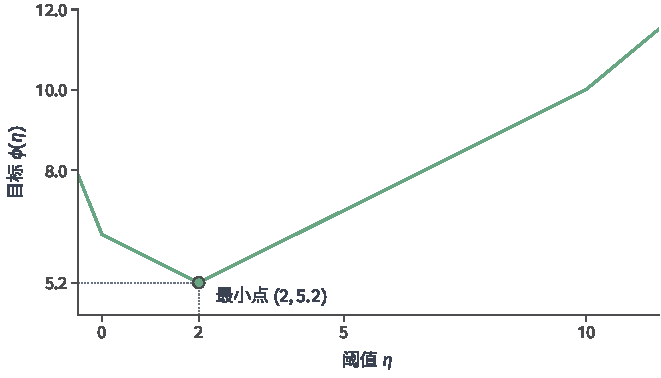
\includegraphics[width=\linewidth]{figures/01-mathematical-preliminaries/05-dynamical-systems-control-decision-and-games/matplotlib/decision-cvar-threshold/figure.pdf}
  \caption{教学分布$P(L=0)=0.6$、$P(L=2)=0.3$、$P(L=10)=0.1$在
  $\alpha=0.75$下的阈值目标$\phi(\eta)=\eta+4\mathbb E[(L-\eta)_+]$。
  绿色折线的最小点为$(2,5.2)$；阈值$2$与尾部平均$5.2$不能混用。}
  \label{fig:decision-cvar-threshold}
\end{figure}

\subsubsection{基于风险包络的尾部评价}

同一个CVaR也可以不用移动阈值，而改成对坏结果增加评价权重。对$L\in L^1(P)$，
\begin{equation}
  \operatorname{CVaR}_\alpha(L)
  =\sup_\zeta\left\{\mathbb E_P[\zeta L]:
    0\leq\zeta\leq\frac{1}{1-\alpha},\quad\mathbb E_P[\zeta]=1\right\}.
  \label{eq:decision-cvar-risk-envelope}
\end{equation}
$\zeta$是相对于原分布的密度比；这些允许密度组成风险包络。
上界$1/(1-\alpha)$阻止全部评价质量压到概率小于$1-\alpha$的事件上。

有限分布中，令结果$i$的原概率为$p_i$、重加权概率为$q_i=p_i\zeta_i$，
右侧变为线性规划
\[
  \max_{\bm q}\sum_iq_iL_i
  \quad\text{s.t.}\quad
  0\leq q_i\leq\frac{p_i}{1-\alpha},\qquad \sum_iq_i=1.
\]
若较小损失仍有质量而较大损失尚未达到上界，将一小部分质量转移到较大损失不会降低
目标。反复转移便得到从最大损失开始填充的解；最后一个损失只取部分质量时，
正是式~\eqref{eq:decision-cvar-atomic-tail}的边界补足。

一般可积分布也能直接证明等式，不必只诉诸形式对偶。对任意可行$\zeta$和$\eta$，
\[
  \mathbb E[\zeta L]
  =\eta+\mathbb E[\zeta(L-\eta)]
  \leq\eta+\frac{\mathbb E[(L-\eta)_+]}{1-\alpha}.
\]
对$\eta$取下确界，说明任意可行密度的加权期望都不超过CVaR。
反向令$q=q_\alpha(L)$，
$b=(1-\alpha)-\mathbb P(L>q)$。若$\mathbb P(L=q)>0$，取
\[
  \zeta^\star=
  \frac{\mathbb I\{L>q\}}{1-\alpha}
  +\frac{b\,\mathbb I\{L=q\}}{(1-\alpha)\mathbb P(L=q)}.
\]
分位条件保证$0\leq b\leq\mathbb P(L=q)$，故密度满足上界且期望为$1$。
若$\mathbb P(L=q)=0$，则$b=0$，只保留第一项。计算
$\mathbb E[\zeta^\star L]$得到原子尾部公式，所以上确界达到CVaR。

例~\ref{ex:decision-cvar-partial-atom}中，损失$10$的原质量$0.1$至多放大为$0.4$，
剩余$0.6$放到损失$2$，重加权为$(0,0.6,0.4)$。
\begin{figure}[htbp]
  \centering
  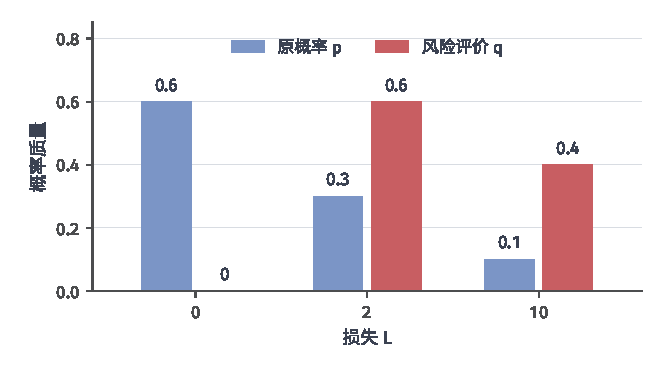
\includegraphics[width=\linewidth]{figures/01-mathematical-preliminaries/05-dynamical-systems-control-decision-and-games/matplotlib/decision-cvar-reweighting/figure.pdf}
  \caption{损失$0,2,10$的名义概率为$(0.6,0.3,0.1)$，CVaR$_{0.75}$的约束为
  $q_i\leq4p_i$和$\sum_iq_i=1$。最优重加权$(0,0.6,0.4)$的期望为$5.2$。
  蓝色为名义质量，红色为对偶最优质量；真实发生概率并未因评价重加权而改变。}
  \label{fig:decision-cvar-reweighting}
\end{figure}

CVaR的相干性质也可从阈值式逐项核对。$L\leq L'$使每个阈值下的正部期望不增，
取下确界得到单调性。将$L+m$的阈值写成$\eta=\bar\eta+m$，便得
$\operatorname{CVaR}_\alpha(L+m)=\operatorname{CVaR}_\alpha(L)+m$。
对$t>0$令$\eta=t\bar\eta$得到正齐次性，$t=0$直接由零损失验证。
又由于
\[
  (L_1+L_2-\eta_1-\eta_2)_+
  \leq(L_1-\eta_1)_++(L_2-\eta_2)_+,
\]
先以$\eta_1+\eta_2$评价合计损失，再分别对两个阈值取下确界，得到次可加性，
继而得到凸性。这些性质都不要求损失分布连续。

这个包络是由既定概率和尾部水平$\alpha$规定的评价权重集合。模型不确定性则问
真实生成机制可能是哪一个分布。二者都能写成最坏期望，但一般不是同一集合，
更不能把重加权结果当作重新估计出的真实事故概率。

\subsection{概率约束与模型不确定性}

有些要求不是把风险再加进目标，而是排除违规概率过大的策略。固定策略产生损失$L$，
给定阈值$b$和$\varepsilon\in(0,1)$，\term{机会约束}（chance constraint）为
\begin{equation}
  \mathbb P(L>b)\leq\varepsilon.
  \label{eq:decision-chance-constraint}
\end{equation}
它控制超标是否发生，不区分超标幅度。由于
$\operatorname{VaR}_{1-\varepsilon}(L)\leq
\operatorname{CVaR}_{1-\varepsilon}(L)$，
条件$\operatorname{CVaR}_{1-\varepsilon}(L)\leq b$蕴含此机会约束。
反向一般不成立，小概率违规的损失可以很大。

必须把违规事件写清楚。温度任务可以限制终端$\{x_H>3\}$、某时刻$\{x_t>3\}$，
也可以限制整段$\{\exists t\leq H:x_t\notin[0,3]\}$。若每个时刻违规概率至多为
$\varepsilon_t$，并集界只给出整段违规概率不超过$\sum_{t=0}^H\varepsilon_t$；
各时刻都不超过$\varepsilon$，不自动使整段也不超过$\varepsilon$。
期望舒适成本很小同样不能替代这些事件保证。

加入输入限制$0\leq u\leq1$和状态限制$0\leq x\leq3$时，先检查可行性。
无噪声下，任意$x\in[0,3]$取$u=0$即可留在区间内，但共同反馈
$u=1-0.3x$还需单独核验：它在区间上取$[0.1,1]$，且下一状态
$x'=0.5x+1\in[1,2.5]$，因此可行。为演示有界扰动下的逐路径安全，
这里将第~\ref{chap:control-theory}章“策略的实现与轨迹控制”中用于矩计算的高斯噪声
改为两点分布；动力学和反馈不变，但噪声假设不同。若$w_{t+1}$独立同分布、等概率取$\pm0.1$，
同一反馈有$x'\in[0.9,2.6]$，仍可保持该区间。这一例取状态完全可见，过程噪声
独立于初态及策略私有随机数。若另有观测噪声$v_t$独立同分布且等概率取$\pm0.05$，
并与过程噪声、初态和私有随机数相互独立，则必须重新检查具体输出反馈；
不能将状态反馈的保证照搬。无界高斯扰动则不能由这种有界输入保证逐路径不越界。

若转移机制由未知$\theta\in\Theta$决定，固定策略的最坏期望是
$\sup_{\theta\in\Theta}\mathbb E^\pi_{P_\theta}[L]$。
\term{分布鲁棒优化}（distributionally robust optimization, DRO）使用候选分布集
$\mathcal P$，相应的评价为$\sup_{Q\in\mathcal P}\mathbb E^\pi_Q[L]$。
距离、矩条件或散度可以规定$\mathcal P$，但集合如何构造和真实分布落入集合的置信保证
仍须分别论证；分布比较工具本身不会自动给出覆盖保证。优化阶段再对允许策略取下确界，
不能在固定策略评价中提前改变行动。

以$L_{\mathrm{safe}}$和$L_{\mathrm{tail}}$为例，$b=10,\varepsilon=0.05$时，
两者违规概率为$0$和$0.05$，都满足机会约束；CVaR$_{0.95}$却为$1$和$20$。
若第二项损失$20$的概率只知$p\in[0.02,0.08]$，最坏期望为
$\max_p20p=1.6$，逐路径最坏损失为$20$，而机会约束在整个集合上不成立，
因为$p=0.08$也被允许。这些数分别描述尾部平均、事故概率、最坏模型平均和路径上界。

有限样本空间中，非空闭候选集位于紧致概率单纯形内，线性期望必达到最大值。
若集合排除某些结果，保证也只覆盖其允许支持。交换策略的$\inf$与模型的$\sup$，
或把内层写成无间隙的对偶，还需凸性、紧致性、连续性或相应约束资格；
最坏分布存在并不够。随机波动、参数估计误差和模型歧义由此得到区分。

\subsection{逐时信息下的动态风险}
\label{sec:decision-dynamic-risk-time-consistency}

\subsubsection{静态尾部评价与偏好反转}

从起点评价整条轨迹，与到达某个分支后重新评价剩余损失，是两个不同操作。
期望有塔式性质把二者连接起来，静态CVaR一般没有同样的关系。
考虑一棵两阶段树：起点等概率进入$N$和$B$，$N$的损失固定为$2$；
在$B$可以预先承诺固定方案$F$或随机方案$R$，
\[
  L_F=3.5,\qquad
  L_R=
  \begin{cases}
    0,&\text{条件概率 }1/2,\\
    4,&\text{条件概率 }1/2.
  \end{cases}
\]
先分别评价这两项承诺策略。承诺$F$时，起点损失以相同概率取$2,3.5$，
所以$\operatorname{CVaR}_{0.5}(L^F)=3.5$。承诺$R$时，起点损失以概率
$1/4,1/2,1/4$取$0,2,4$，故
\[
  \operatorname{CVaR}_{0.5}(L^R)
  =\frac{(1/4)\times4+(1/4)\times2}{1/2}=3.
\]
静态评价因此偏好$R$。真正到达$B$后，只在该条件分布内重算同一水平的CVaR，
却有
\[
  \operatorname{CVaR}_{0.5}(L_F\mid B)=3.5,\qquad
  \operatorname{CVaR}_{0.5}(L_R\mid B)=4,
\]
排序反转。起点评价时，$N$的损失占用了静态尾部的一部分；条件化后，未到达的$N$
已经排除。反转不是算错，而是整条轨迹的尾部与当前分支的尾部并非同一批结果。

\begin{table*}[htbp]
  \centering
  \begin{tabularx}{\linewidth}{XccX}
    \toprule
    评价口径 & 承诺$F$ & 承诺$R$ & 比较依据\\
    \midrule
    初始静态$\operatorname{CVaR}_{0.5}$ & $3.5$ & $3$ & 整棵树最坏一半的损失\\
    到达$B$后的条件$\operatorname{CVaR}_{0.5}$ & $3.5$ & $4$ & $B$内最坏一半的损失\\
    两层嵌套$\operatorname{CVaR}_{0.5}$ & $3.5$ & $4$ & 先评价子节点，再评价节点风险\\
    \bottomrule
  \end{tabularx}
  \caption{同一两阶段分布的三种评价。根节点等概率到达$N$或$B$，$N$固定损失为$2$。
  前两行发生偏好反转；第三行使用下节定义的嵌套目标，其数值不等于静态总损失CVaR。}
  \label{tab:decision-static-conditional-nested}
\end{table*}

\subsubsection{条件风险与时间一致性}

要在每次增加信息后按同一规则评价剩余损失，可以明确规定：下一节点先给出风险值，
当前节点再汇总这些值。令$\mathcal F_0\subseteq\cdots\subseteq\mathcal F_H$
为逐时增长的信息；阈值等评价参数只能使用当时已知的信息。
\begin{definition}[一步条件风险映射]
\label{def:decision-conditional-risk-mapping}
在同一概率空间上，一步\term{条件风险映射}（conditional risk mapping）
\[
  \rho_t:L^\infty(\mathcal F_{t+1})\longrightarrow L^\infty(\mathcal F_t)
\]
把下一时刻可知的有界随机损失转成当前信息下的风险。输入与输出均按几乎处处相等的
等价类理解。
\end{definition}
常用条件为单调性、当前信息下的平移等变性和归一化：
\begin{align}
  Z\leq Z'&\ \Longrightarrow\ \rho_t(Z)\leq\rho_t(Z'),
  \label{eq:decision-conditional-risk-monotonicity}\\
  \rho_t(Z+M)&=\rho_t(Z)+M,\qquad M\in L^\infty(\mathcal F_t),
  \label{eq:decision-conditional-risk-translation}\\
  \rho_t(0)&=0.\notag
\end{align}
条件期望满足这些条件。有限树上逐节点评价的映射还具有局部性：若事件
$E\in\mathcal F_t$，只改变$E$之外的未来损失，不改变$E$内的评价。
一般条件模型使用节点解释时也须保持这种信息适应性。

条件CVaR为
\begin{equation}
  \operatorname{CVaR}_{\alpha,t}(Z)
  =\operatorname*{ess\,inf}_{\eta\in L^\infty(\mathcal F_t)}
    \left\{\eta+\frac{1}{1-\alpha}
      \mathbb E[(Z-\eta)_+\mid\mathcal F_t]\right\}.
  \label{eq:decision-conditional-cvar}
\end{equation}
$\eta$可随当前历史改变，不能偷看未来结果。
记花括号中的$\mathcal F_t$可测随机变量为$\Phi_\eta$。
这里的本质下确界（essential infimum）是在几乎处处大小关系下最大的共同下界：
它是$\mathcal F_t$可测的随机变量$U$，对每个$\eta$都有$U\leq\Phi_\eta$几乎处处；
任何同样对每个$\eta$满足$V\leq\Phi_\eta$的$\mathcal F_t$可测随机变量$V$，
都必须满足$V\leq U$几乎处处。
因此结果仍随当前历史变化，并不是对全部历史再取一个常数最小值。
这个定义直接在随机变量的几乎处处等价类之间比较，避免把不可数多个版本逐点取下确界时的可测性问题藏起来。
有限概率树上，就是在每个当前节点对其条件分布使用静态阈值公式。
例如固定前例的承诺$R$，在节点$N$与$B$得到的条件风险分别为$2$与$4$。

\begin{definition}[嵌套动态风险]
\label{def:decision-nested-dynamic-risk}
设$C_t\in L^\infty(\mathcal F_t)$为当前已知的有界损失，给定一步映射$(\rho_t)$，
由终端向前定义
\begin{align}
  \mathcal R_H(C_H)&=C_H,\notag\\
  \mathcal R_t(C_t,\ldots,C_H)
  &=C_t+\rho_t\bigl(\mathcal R_{t+1}(C_{t+1},\ldots,C_H)\bigr).
  \label{eq:decision-nested-dynamic-risk}
\end{align}
称为\term{嵌套动态风险}（nested dynamic risk）。
\end{definition}
这里当前成本在风险映射外，是因为它已经属于$\mathcal F_t$。
若成本$\widetilde C_{t+1}$到下一时刻才揭晓，则应写成
\[
  \widetilde{\mathcal R}_t
  =\rho_t(\widetilde C_{t+1}+\widetilde{\mathcal R}_{t+1}).
\]
随机行动尚未抽取时，依赖该行动的阶段成本也属于尚未揭晓的量，不能无条件提出。

\begin{definition}[递归意义下的时间一致性]
\label{def:decision-time-consistency}
动态风险族$(\mathcal R_t)$具有\term{时间一致性}（time consistency），是指对每个
$t<H$、任意两组从$t+1$开始的有界适应损失和同一当前损失$C_t$，只要
$\mathcal R_{t+1}(C_{t+1:H})\leq\mathcal R_{t+1}(C'_{t+1:H})$几乎处处成立，
就有$\mathcal R_t(C_t,C_{t+1:H})\leq\mathcal R_t(C_t,C'_{t+1:H})$几乎处处成立。
\end{definition}
它要求下一时刻每个可能历史上的共同排序在当前仍被保留，而不是要求某个单一实现
总能沿用起点的无条件排序。嵌套结构下，若每个$\rho_t$单调，则
\[
  C_t+\rho_t\bigl(\mathcal R_{t+1}(C_{t+1:H})\bigr)
  \leq
  C_t+\rho_t\bigl(\mathcal R_{t+1}(C'_{t+1:H})\bigr),
\]
正是所需结论。相同当前损失这个条件不可删除，否则当前多付的成本本身就可能逆转比较。

回到两节点例，先固定承诺$F$或$R$。在$B$分别得到风险值$3.5$或$4$，
在$N$均为$2$；根节点再对这两个等概率节点值计算CVaR$_{0.5}$，
得到$3.5$或$4$。所以嵌套评价偏好$F$，静态评价偏好$R$。
递归结构保证了上述时间一致性，但没有把两个不同目标变成同一目标的两种算法。

\section{策略的轨迹价值计算}
\label{sec:policy-value-evaluation}

\subsection{有限时域下的价值递推}
\label{sec:policy-finite-evaluation}

固定策略后，价值计算不再选择行动，而是把该规则可能产生的未来后果逐层汇总。
有限时域从终端开始最直接：$V_H^\pi(s)=c_H(s)$。对于给定Markov策略，
先对下一状态条件化，再按已经指定的行动概率平均，得到
\begin{equation}
  V_t^\pi(s)=\sum_a\pi_t(a\mid s)
  \left[c_t(s,a)+\sum_{s'}P_t(s'\mid s,a)V_{t+1}^\pi(s')\right].
  \label{eq:decision-policy-bellman}
\end{equation}
这就是固定策略的Bellman评价式。若下一时刻的价值已算出，一次矩阵求和即可把
时刻$t$的价值算出；没有任何$\min_a$。

其依据是塔式法则。把累计和拆成$c_t(S_t,A_t)$与后续和，在$S_t=s,A_t=a$
下对后续和条件化，其期望为
$\sum_{s'}P_t(s'\mid s,a)V_{t+1}^\pi(s')$；
再对$\pi_t(a\mid s)$求和，得到上式。归纳到$t=0$后，
$J^\pi=\sum_s\mu_0(s)V_0^\pi(s)$。对一般历史策略，同样的证明给出
\[
  J_t^\pi(h_t)=\sum_a\pi_t(a\mid h_t)
  \left[c_t(s,a)+\sum_{s'}P_t(s'\mid s,a)
    J_{t+1}^\pi(h_t,a,s')\right].
\]
只有当继续规则与所需预测信息都由当前状态概括时，才可把$J_t^\pi(h_t)$缩写为
$V_t^\pi(s)$。Markov环境不意味着任意历史策略本身自动变成Markov策略。

在路线例中，固定以概率$p$走捷径的策略有
\[
  V_0^\pi(s_0)=(1-p)\times2+p(0.8\times0+0.2\times6)=2-0.8p.
\]
$p=1/2$给出$1.6$。这与按三条轨迹概率$(0.5,0.4,0.1)$直接求和一致。
递推省去了枚举长轨迹的代价，却没有改变评价对象。

\begin{example}[温度策略的两步成本]
\label{ex:policy-temperature-evaluation}
取式~\eqref{eq:policy-temperature-model}无噪声、$x_0=0,H=2$，
并按式~\eqref{eq:policy-temperature-cost}计价。固定反馈
$u_t=0.4-0.3(x_t-2)$得到
$(x_0,x_1,x_2)=(0,1,1.5)$、$(u_0,u_1)=(1,0.7)$。
由终端向前，
\begin{align*}
  V_2^\pi(1.5)&=0.25,\\
  V_1^\pi(1)&=1+0.49+0.25=1.74,\\
  V_0^\pi(0)&=4+1+1.74=6.74.
\end{align*}
舒适偏差合计$4+1+0.25=5.25$，输入平方合计$1+0.49=1.49$。
另一项固定策略始终取$u_t=0.4$，产生$(0,0.4,0.72)$，其成本为
\[
  4+1.6^2+1.28^2+0.4^2+0.4^2=8.5184.
\]
其中舒适成本为$8.1984$，输入成本为$0.32$。所以在这个初态、两步时域和给定权重下，
反馈策略用更多输入换来更小的总成本；对应累计收益为$-6.74$和$-8.5184$。
这个比较只涉及两项指定策略，并没有证明第一项在所有策略中最优。
\end{example}

图~\ref{fig:policy-temperature-comparison}将上述评价并列展示：状态更快接近目标，
并不意味着每一项成本都较低。反馈增加了输入成本，但在这两步内节省了更多舒适成本。
\begin{figure*}[htbp]
  \centering
  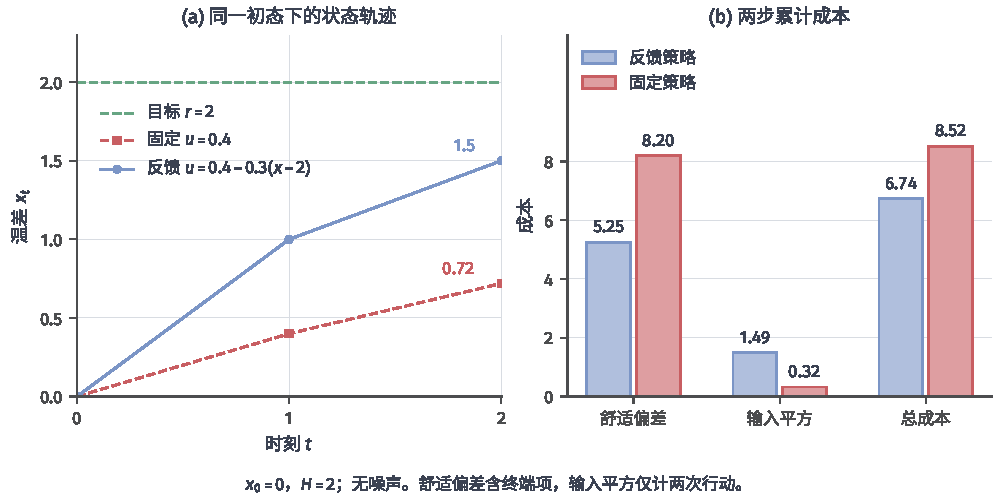
\includegraphics[width=\linewidth]{figures/01-mathematical-preliminaries/05-dynamical-systems-control-decision-and-games/matplotlib/policy-temperature-comparison/figure.pdf}
  \caption{共同温度模型下两项固定策略的比较。左图连接离散时刻的状态，绿色虚线为
  目标温差$2$；连线仅用于辨认轨迹，不表示额外的连续时间模型。右图按
  $c(x,u)=(x-2)^2+u^2$和终端成本$(x-2)^2$累计，柱顶数值保留两位小数。
  反馈的精确总成本为$6.74$，固定输入的总成本为$8.5184$。先分别求值再比较，
  并未在每一步重新选择最优行动。}
  \label{fig:policy-temperature-comparison}
\end{figure*}

恢复随机扰动后，同一反馈诱导轨迹分布而非上述单一路径。若成本可积，
可以沿条件分布求期望；不能只把噪声取均值零后代回非线性的平方成本。
例如$\mathbb E[(x-r)^2]=(\mathbb E[x]-r)^2+\operatorname{Var}(x)$，
漏掉方差项就低估了舒适成本。

\subsection{无限折扣时域下的价值计算}
\label{sec:policy-discounted-evaluation}

有限时域有一个可以启动反向计算的终端，无限时域则没有最后一步。
折扣和有界成本使远期影响可控，由此可把评价转化为固定点计算。
以下取有限状态行动、时不变转移、$|c(s,a)|\leq C$、
$0\leq\gamma<1$和给定的平稳Markov策略$\pi$。定义
\[
  c^\pi(s)=\sum_a\pi(a\mid s)c(s,a),\qquad
  P^\pi(s,s')=\sum_a\pi(a\mid s)P(s'\mid s,a),
\]
以及固定策略评价算子
\begin{equation}
  (T^\pi V)(s)=c^\pi(s)+\gamma\sum_{s'}P^\pi(s,s')V(s').
  \label{eq:policy-discounted-evaluation-operator}
\end{equation}
由$P^\pi(s,s')$组成的矩阵每行非负且和为$1$，所以对任意两个价值函数，
\[
  |(T^\pi V)(s)-(T^\pi W)(s)|
  \leq\gamma\sum_{s'}P^\pi(s,s')|V(s')-W(s')|
  \leq\gamma\lVert V-W\rVert_\infty.
\]
取状态最大值便得到$\gamma$-压缩。有限维最大范数空间完备，压缩映射定理给出
唯一固定点。另一方面，折扣成本的绝对和不超过$C/(1-\gamma)$，
可合法拆出第一项并条件化，得到$V^\pi=T^\pi V^\pi$。
因此这个唯一固定点正是指定策略的期望累计成本，不是最优成本。

从任意$V^{(0)}$出发令$V^{(k+1)}=T^\pi V^{(k)}$，有
\begin{equation}
  \lVert V^{(k)}-V^\pi\rVert_\infty
  \leq\gamma^k\lVert V^{(0)}-V^\pi\rVert_\infty.
  \label{eq:policy-evaluation-iteration-error}
\end{equation}
若取$V^{(0)}=0$，右侧可用$\gamma^kC/(1-\gamma)$替代。
不知$V^\pi$时，也可用可计算残差
\[
  \lVert V-V^\pi\rVert_\infty
  \leq\frac{\lVert T^\pi V-V\rVert_\infty}{1-\gamma},
\]
因为三角不等式和压缩性给出
$\lVert V-V^\pi\rVert_\infty\leq
\lVert V-T^\pi V\rVert_\infty+\gamma\lVert V-V^\pi\rVert_\infty$。
这提供停止评价迭代的误差证书。

将$c^\pi(s),V^\pi(s)$排列为列向量$\bm c^\pi,\bm V^\pi$，以
$P^\pi(s,s')$为元素组成矩阵$\bm P^\pi$，则
\[
  \bm V^\pi=(\bm I-\gamma\bm P^\pi)^{-1}\bm c^\pi
  =\sum_{j=0}^\infty\gamma^j(\bm P^\pi)^j\bm c^\pi.
\]
无穷级数在最大范数下收敛，故逆矩阵存在。单状态例中，
若策略每步以概率$1/4$选择成本$4$的行动，其余选择成本$0$的行动，
则$c^\pi=1$；$\gamma=0.9$时$V^\pi=10$，从零开始迭代得到
$V^{(k)}=10(1-0.9^k)$。这里平均的是固定行动分布；
若把每步成本改成两行动中较小的$0$，算出的已是另一个优化问题。

非平稳或一般历史策略仍有定义良好的有界折扣价值，但其继续规则可能随时间或历史变化，
不能直接使用这个单一平稳算子。可以保留时间、扩充状态，或对有限截断时域评价后
控制余项。连续状态无界二次成本也需要另行选择函数空间与矩条件。

\subsection{风险评价下的价值计算}

\subsubsection{嵌套风险下的递推计算}
\label{sec:policy-nested-risk-evaluation}

先固定确定性Markov策略$a=\pi_t(s)$。若当前状态确实包含风险评价所需的信息，
一步风险映射可写为$\rho_{t,s,a}$，它作用于按$P_t(\cdot\mid s,a)$分布的下一状态。
从终端开始计算
\[
  V_H^{\pi,\rho}(s)=c_H(s),\qquad
  V_t^{\pi,\rho}(s)
  =c_t(s,\pi_t(s))+
    \rho_{t,s,\pi_t(s)}\bigl(V_{t+1}^{\pi,\rho}(S_{t+1})\bigr).
\]
其含义与定义~\ref{def:decision-nested-dynamic-risk}完全一致：先接受后续节点的
评价，再按当前节点风险汇总。策略仍固定，不从其他行动中挑更小的一个。

随机策略需要多说明一层。采取行动之前，$A_t$尚未揭晓；
可在联合条件分布
$\pi_t(a\mid s)P_t(s'\mid s,a)$上，对行动和下一状态一起评价：
\begin{equation}
  V_t^{\pi,\rho}(s)=
  \rho^\pi_{t,s}\bigl(c_t(s,A_t)+V_{t+1}^{\pi,\rho}(S_{t+1})\bigr).
  \label{eq:policy-joint-action-risk-evaluation}
\end{equation}
这里$\rho^\pi_{t,s}$的输入是$(A_t,S_{t+1})$上的随机损失，连当前阶段成本也必须
放在映射内。另一种明确可定义的目标，是先对每个已选行动的环境后果计算风险，
再对行动随机化使用期望：
\[
  \overline V_t^{\pi,\rho}(s)=\sum_a\pi_t(a\mid s)
    \left[c_t(s,a)+\rho_{t,s,a}
      \bigl(\overline V_{t+1}^{\pi,\rho}(S_{t+1})\bigr)\right].
\]
这个公式不是从前式用线性性推出来的，而是改变了行动随机性的评价口径。
路线策略$p=1/2$时，联合损失概率为$0.4$取$0$、$0.5$取$2$、$0.1$取$6$，
联合CVaR$_{0.9}$为$6$；先分别算行动的CVaR再平均，得到
$\tfrac12\times2+\tfrac12\times6=4$。期望下两种次序相同，非线性风险下通常不同。

误差控制依靠单调性和平移等变性，而不依靠线性性。设有限状态上的
$\lVert V-W\rVert_\infty\leq\delta$，则
$W(S')-\delta\leq V(S')\leq W(S')+\delta$，因此
\[
  \rho_{s,a}(W(S'))-\delta
  \leq\rho_{s,a}(V(S'))
  \leq\rho_{s,a}(W(S'))+\delta.
\]
每个映射在最大范数下非扩张。有限时域中一次评价误差不会被单步放大；
若第$t$步另引入至多$\epsilon_t$的数值误差，则反向传播后的初始误差至多为
终端误差加$\sum_{t=0}^{H-1}\epsilon_t$。

无限时域可明确选用“折扣后续风险值”的递归目标。固定确定策略的算子为
\[
  (T^\pi_\rho V)(s)
  =c(s,\pi(s))+\gamma\rho_{s,\pi(s)}(V(S')).
\]
归一化、单调和平移等变保证它把有界向量映到有界向量，且为$\gamma$-压缩，
因而有唯一固定点，迭代误差与残差界分别为
$\gamma^k\lVert V^{(0)}-V^{\pi,\rho}\rVert_\infty$和
$\lVert T^\pi_\rho V-V\rVert_\infty/(1-\gamma)$。
后续风险乘$\gamma$是本目标的明确约定；对CVaR等正齐次风险，它也等于
$\rho_{s,\pi(s)}(\gamma V(S'))$。一般凸风险不一定允许把$\gamma$移入或移出。
若使用随机行动的联合目标
$\rho^\pi_s(c(s,A)+\gamma V(S'))$，相同非扩张论证仍给出$\gamma$-压缩，
但它是该联合目标自己的固定点，不能与前一个目标混称。

上述证明中的$V,W$是有限状态上的实际向量。推广到一般$L^\infty$等价类时，
还须保证转移核不会读取所选代表在零测集上的任意值；有限状态的最大范数论证
不能未经核对直接替换成本质上确界版本。

风险包络进一步解释这项计算何时等价于局部最坏模型。先在有$m$个结果的有限空间上
取相干风险$\rho:\mathbb R^m\to\mathbb R$，定义
\[
  \mathcal Q=\{\bm q\in\mathbb R^m:
    \langle\bm q,\bm z\rangle\leq\rho(\bm z)
    \text{ 对所有 }\bm z\in\mathbb R^m\}.
\]
正齐次与次可加使$\rho$为有限次线性函数。其凸共轭在$\mathcal Q$上为零，
在其外为无穷：若某个$\bm z$违反支撑不等式，将$\bm z$放大即使共轭发散。
有限凸函数连续，Fenchel--Moreau表示因而给出
$\rho(\bm z)=\sup_{\bm q\in\mathcal Q}\langle\bm q,\bm z\rangle$。
将$r\bm 1$代入支撑不等式，并令$r$取任意正负值，平移等变性迫使
$\langle\bm q,\bm1\rangle=1$；若$q_i<0$，取$\bm z=-r\bm e_i$且$r>0$，
单调性给出$\rho(\bm z)\leq\rho(0)=0$，却有
$\langle\bm q,\bm z\rangle>0$，矛盾。因此$q_i\geq0$。
支撑表示保证集合非空，且它是概率单纯形中的闭凸集，所以紧致，最大值达到。

一般归一化、单调、平移等变的凸风险未必正齐次，其对偶为
\[
  \rho(\bm z)=\sup_{\bm q\in\Delta_m}
  \{\langle\bm q,\bm z\rangle-\beta(\bm q)\},\qquad
  \Delta_m=\{\bm q\geq0:\langle\bm q,\bm1\rangle=1\}.
\]
$\beta$是可取无穷的凸罚函数，不能无条件删去。相干一步映射则有
\begin{equation}
  \rho_{s,a}(V(S'))
  =\sup_{q\in\mathcal Q(s,a)}
    \sum_{s'}q(s'\mid s,a)V(s').
  \label{eq:decision-one-step-risk-envelope}
\end{equation}
条件CVaR对应相对于名义转移的有界密度比。固定策略后逐步代入这些包络，
究竟是否等于原先声明的整条轨迹最坏期望，还取决于各节点的模型选择能否自由拼接。

\begin{definition}[条件分布集合的矩形性]
\label{def:decision-rectangular-uncertainty}
在有限概率树上，为每个历史行动节点给定非空下一步条件分布集合。若允许的路径分布
恰好包括从各节点集合任意选取条件核，再按路径相乘得到的全部分布，则称该不确定集合
具有\term{矩形性}（rectangularity）。
\end{definition}
Markov表达中可使用$\mathcal Q(s,a)$，但模型的局部选择仍可依赖已发生历史，
且不受“其他节点必须使用同一个未知参数”等跨节点约束。固定策略不变时，
逆向归纳说明矩形集合的最坏期望可逐节点求得：最末节点选其最坏条件分布；
前一节点对这些已取得的继续值取最坏期望；矩形性保证各节点的选择能拼成同一允许
路径模型。反过来，任一允许模型的局部期望不超过该局部上确界，逐步回代得到上界。
有限树和紧致局部包络保证所有最大值同时可达；没有达到性时可改用近似最坏选择。
这一证明没有改变策略，也没有加入行动最小化。

若一个未知参数全程固定，矩形性通常不成立。设$Y_1,Y_2\in\{0,1\}$在给定
$p\in\{0.2,0.8\}$后独立，两次共用该$p$。原模型下
\[
  \mathbb P_p(Y_1=1,Y_2=0)=p(1-p)=0.16.
\]
若每个节点可独立取最坏$p$，第一步选$0.8$，看到$Y_1=1$后第二步改选$0.2$，
则该事件概率为$0.8\times0.8=0.64$。这个概率不属于任何原来的固定参数模型。
局部递推实际扩大了候选机制，不能称为对原问题的精确求值。
可以保留共享参数约束，或在有先验的模型中更新其信念并扩充状态；
单纯把一个集合名称写进Bellman式不会消除跨时耦合。

\subsubsection{静态尾部风险下的增广计算}
\label{sec:policy-static-cvar-evaluation}

如果仍然要评价起点处的静态总损失CVaR，就不应更换成嵌套目标。
以有限时域折扣损失
$L=\sum_{t=0}^{H-1}\gamma^tc_t(S_t,A_t)+\gamma^Hc_H(S_H)$为例，
这里也允许$\gamma=1$。固定策略$\pi$和阈值$\eta$后，需要计算的是
$\mathbb E^\pi[(L-\eta)_+]$。同一物理状态可能由不同历史到达，已经累计的损失不同，
越过阈值的剩余空间也不同，因此原状态通常不够。

把已累计成本记为$B_0=0$、
$B_{t+1}=B_t+\gamma^tc_t(S_t,A_t)$。
若固定策略为$\pi_t(a\mid s,b)$，定义在增广状态上的终端与递推
\begin{align}
  W_H^{\pi,\eta}(s,b)&=(b+\gamma^Hc_H(s)-\eta)_+,\notag\\
  W_t^{\pi,\eta}(s,b)
  &=\sum_a\pi_t(a\mid s,b)\sum_{s'}P_t(s'\mid s,a)
    W_{t+1}^{\pi,\eta}\bigl(s',b+\gamma^tc_t(s,a)\bigr).
  \label{eq:policy-static-cvar-augmented-evaluation}
\end{align}
这仍是普通条件期望评价，正部非线性全部留在终端。原Markov策略是这里不依赖$b$
的特例；若给定策略还读取未被$(s,b)$保留的历史，就继续保留那部分历史，
不能因成本已增广而擅自改写原策略。

计算完每个阈值的期望以后，该固定策略的风险为
\[
  \operatorname{CVaR}_\alpha(L^\pi)
  =\inf_{\eta\in\mathbb R}
    \left\{\eta+\frac{1}{1-\alpha}
      \sum_s\mu_0(s)W_0^{\pi,\eta}(s,0)\right\}.
\]
这里优化$\eta$只是计算CVaR定义中的辅助参数，并没有优化策略。
例如在累计成本$b=0$或$b=5$时都到达同一零终端成本状态，阈值$\eta=3$对应
正部损失$0$和$2$，足见只记录物理状态无法作相同的终端结算。
增广状态可能连续，计算规模会增加；无界成本需要正部期望有限。
下一节才允许策略随增广状态改变，并说明这时阈值与策略如何联合优化。

\section{策略的轨迹价值优化}
\label{sec:policy-value-optimization}

前一节对指定行动规则求值，现在才把规则本身作为变量。最优性总是相对于允许信息、
可行行动和既定准则而言：降低期望成本不保证每条实现轨迹都更好，也不自动保证安全。
单步选择先展示“按后果比较行动”，多步问题再把后果换成当前成本加最优继续价值。

\subsection{单步价值下的行动选择}
\label{sec:decision-bayes-rules}

只有一次行动时，轨迹损失退化为$\ell(a,Y)$。设观测为$X$，未知结果
$Y\in\mathcal Y$，可选行动$a\in\mathcal A$，损失
$\ell:\mathcal A\times\mathcal Y\to\mathbb R$给出每种行动在每种结果下的代价。
结果未揭晓前不能逐列挑选最低损失，只能依据当前可用的条件分布选择一整项行动。

\begin{definition}[条件风险与Bayes决策]
\label{def:decision-conditional-risk-bayes-rule}
给定条件分布核$P(\mathrm dy\mid x)$，假设损失可测且下列期望有限。
行动$a$在观测$x$下的\term{条件风险}（conditional risk）为
\begin{equation}
  r(a\mid x)=\mathbb E[\ell(a,Y)\mid X=x]
  =\int_{\mathcal Y}\ell(a,y)P(\mathrm dy\mid x).
  \label{eq:decision-conditional-risk}
\end{equation}
若最小值达到，任取
\begin{equation}
  a^\star(x)\in\argmin_{a\in\mathcal A}r(a\mid x)
  \label{eq:decision-bayes-action}
\end{equation}
称为\term{Bayes行动}（Bayes action）。若该选择关于$x$可测，
映射$\delta^\star(x)=a^\star(x)$称为\term{Bayes决策规则}（Bayes decision rule）。
\end{definition}
有限类别时，积分就是$\sum_y\ell(a,y)p(y\mid x)$。这里“Bayes”指按照给定
条件分布最小化期望损失；该分布可以由先验和似然更新，也可以由其他概率模型给出。
Bayes公式更新信念，Bayes规则把信念转成行动，二者不是同一步。

可测规则$\delta$的总体风险为
\begin{equation}
  R(\delta)=\mathbb E[\ell(\delta(X),Y)].
  \label{eq:decision-rule-risk}
\end{equation}
塔式法则和逐点最小性给出完整的总体比较：
\[
  R(\delta^\star)
  =\mathbb E\!\left[\mathbb E[\ell(\delta^\star(X),Y)\mid X]\right]
  =\mathbb E[\min_a r(a\mid X)]
  \leq\mathbb E[r(\delta(X)\mid X)]
  =R(\delta).
\]
期望存在和可测选择不可省略。有限行动可以按固定次序处理并列；连续行动还要检查
成本的可测性、下半连续性及最小值达到条件，否则下确界未必对应一项可实施规则。

\begin{example}[有限损失表的逐项计算]
\label{ex:decision-finite-loss-table}
设$Y\in\{y_0,y_1\}$，损失表为
\[
  \begin{array}{c|cc}
    &y_0&y_1\\ \hline
    a_0&0&6\\
    a_1&2&1
  \end{array}
\]
若$\mathbb P(Y=y_1\mid X=x)=1/4$，则
\[
  r(a_0\mid x)=\frac34\times0+\frac14\times6=\frac32,\qquad
  r(a_1\mid x)=\frac34\times2+\frac14\times1=\frac74.
\]
Bayes行动是$a_0$。比较的是各整行的概率加权损失，不能先观察尚未知的结果，
再在每列选较小数字。一般有限结果$\{y_1,\ldots,y_m\}$使用
$r(a\mid x)=\sum_{j=1}^m\ell(a,y_j)\mathbb P(Y=y_j\mid X=x)$。
\end{example}

非对称错误代价会改变同一预测概率对应的行动。二分类中令
$p(x)=\mathbb P(Y=1\mid X=x)$，正确预测损失为零，假阳性和假阴性损失分别为
$c_{\mathrm{FP}}>0,c_{\mathrm{FN}}>0$。两行动风险为
\begin{align}
  r(1\mid x)&=c_{\mathrm{FP}}(1-p(x)),
  \label{eq:decision-binary-risk-positive}\\
  r(0\mid x)&=c_{\mathrm{FN}}p(x).
  \label{eq:decision-binary-risk-negative}
\end{align}
预测阳性当且仅当第一项不大于第二项，即
\begin{equation}
  p(x)\geq\frac{c_{\mathrm{FP}}}{c_{\mathrm{FP}}+c_{\mathrm{FN}}}.
  \label{eq:decision-cost-sensitive-threshold}
\end{equation}
等号处风险并列，可按约定处理。错误代价相同时阈值为$1/2$；漏诊代价增加使阈值下降。
概率模型并未变化，变化的是对后果的计价。概率校准良好不能替代正确损失设定。

\begin{example}[同一概率对应不同合理行动]
\label{ex:decision-same-probability-different-actions}
设$p(x)=0.3$。对称零一损失的阈值为$0.5$，应预测阴性。
若漏诊损失为$9$、误报损失为$1$，阈值变为$1/(1+9)=0.1$，应预测阳性。
这些教学数值只说明概率之外还需要价值判断，不为具体应用决定真实代价。
\end{example}

图~\ref{fig:decision-cost-thresholds}把行动比较画成两条风险曲线的下包络。
“更谨慎”必须说明针对哪一种错误，才能判断阈值往哪里移动。
\begin{figure*}[htbp]
  \centering
  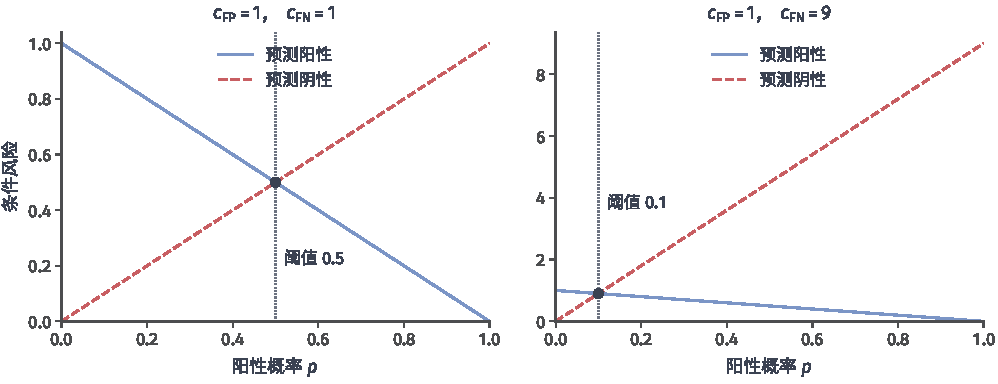
\includegraphics[width=\linewidth]{figures/01-mathematical-preliminaries/05-dynamical-systems-control-decision-and-games/matplotlib/decision-cost-thresholds/figure.pdf}
  \caption{二分类的条件风险。蓝色实线是预测阳性的$c_{\mathrm{FP}}(1-p)$，
  红色虚线是预测阴性的$c_{\mathrm{FN}}p$。左图两种错误成本均为$1$，阈值$0.5$；
  右图漏诊成本增至$9$，阈值降为$0.1$。横轴相同，纵轴分别显示各自损失范围。}
  \label{fig:decision-cost-thresholds}
\end{figure*}

允许拒答时，行动集合又发生改变。令类别为$\{1,\ldots,K\}$，分类采用零一损失，
增加拒答行动$\bot$，其成本为$c_{\mathrm R}\in(0,1)$。
最可能类别的条件错误风险为$1-p_{\max}(x)$，其中
$p_{\max}(x)=\max_k\mathbb P(Y=k\mid X=x)$。与拒答成本比较得
\begin{equation}
  \delta^\star(x)=
  \begin{cases}
    \argmax_k\mathbb P(Y=k\mid X=x),&p_{\max}(x)\geq1-c_{\mathrm R},\\
    \bot,&p_{\max}(x)<1-c_{\mathrm R}.
  \end{cases}
  \label{eq:decision-reject-rule}
\end{equation}
类别并列仍按固定次序选择。拒答是有自身代价的行动，不是结果分布中的新类别。
定义\term{覆盖率}（coverage）和正覆盖率下的接受风险
\[
  \operatorname{Coverage}(\delta)=\mathbb P\{\delta(X)\neq\bot\},\qquad
  R_{\mathrm{acc}}(\delta)
  =\mathbb E[\ell(\delta(X),Y)\mid\delta(X)\neq\bot].
\]
这里的覆盖率是接受行动的输入比例；第~\ref{sec:probability-exchangeability-conformal-ranks}节
预测集合的覆盖率$\mathbb P\{Y\in C(X)\}$则衡量集合包含真实响应的概率。
两者使用同一名称，但判断的事件不同。
多拒绝样本可以降低接受风险，所以必须同时报告覆盖率。
固定拒答成本最小化的是包含拒答损失的总体风险，不等于任意指定覆盖率下的
接受风险最小化。

人工复核预算会耦合不同观测点。若要求覆盖率至少为$\kappa$，问题为
\[
  \min_\delta R(\delta)
  \quad\text{s.t.}\quad\mathbb P\{\delta(X)\neq\bot\}\geq\kappa.
\]
在适当条件下，拉格朗日乘子可以把覆盖预算换成拒答的影子价格，仍产生阈值规则，
但阈值由整体分布和预算决定。\term{选择性预测}（selective prediction）选择在哪些
输入上行动，不等同于增大某类错误的代价。

\begin{example}[覆盖预算耦合两个观测点]
\label{ex:decision-two-point-coverage-budget}
设$X$等概率取$x_1,x_2$，两处最优分类错误风险为$0.2,0.4$，拒答损失均为$0.1$。
逐点无约束规则会全部拒答，覆盖率为零。要求覆盖率至少$1/2$且使用确定规则时，
至少接受一个点。接受$x_1$、拒答$x_2$的总体风险为
$\tfrac12\times0.2+\tfrac12\times0.1=0.15$；反向安排为
$\tfrac12\times0.1+\tfrac12\times0.4=0.25$；全部接受为$0.3$。
因此应把有限接受量安排在$x_1$。预算使两个观测点不能再独立执行原拒答规则。
\end{example}

若观测和行动有限，并允许按每个观测的行动概率优化，风险与覆盖约束都是线性的，
得到线性规划，强对偶提供影子价格。只允许确定规则时，选择变量带零一约束，
一般成为整数规划，不能套用普通LP强对偶。连续分布或非凸策略类还要检查可行性、
闭性与约束资格，不能仅写出乘子就宣称不存在对偶间隙。

最后核对随机化本身的作用。给定$x$，按概率核$q(\mathrm da\mid x)$选行动的风险为
\[
  \int_{\mathcal A}r(a\mid x)q(\mathrm da\mid x)\geq\inf_a r(a\mid x).
\]
有限或可数行动时就是加权和。没有额外耦合约束，随机化不能优于最佳纯行动；
最小值达到时，只有将概率放在最优行动上才保持最优。总体预算、公平或资源约束下，
随机化可实现确定规则达不到的平均比例，其作用来自可行域，不是期望损失偏好掷硬币。

\subsection{离散演化下的策略优化}
\label{sec:decision-dynamic-programming}

\subsubsection{有限时域下的最优策略递推}

多步任务中，行动的“损失表”要把后续机会也计入。先计算最后一步可以达到的最小成本，
再用它评价前一步行动，就得到
\begin{align}
  V_H^\star(s)&=c_H(s),
  \label{eq:decision-finite-bellman-terminal}\\
  V_t^\star(s)&=\min_{a\in\mathcal A(s)}
    \left\{c_t(s,a)+\sum_{s'}P_t(s'\mid s,a)V_{t+1}^\star(s')\right\}.
  \label{eq:decision-finite-bellman}
\end{align}
与固定评价式~\eqref{eq:decision-policy-bellman}相比，这里才出现行动最小化；
被最小化的是当前成本与继续价值之和，不只是当前成本。

图~\ref{fig:bellman-evaluation-versus-optimization}将固定策略评价与最优递推并列：两边都先对随机后继价值取期望，再分别按策略平均或在行动之间取最小值。

\begin{figure*}[htbp]
  \centering
  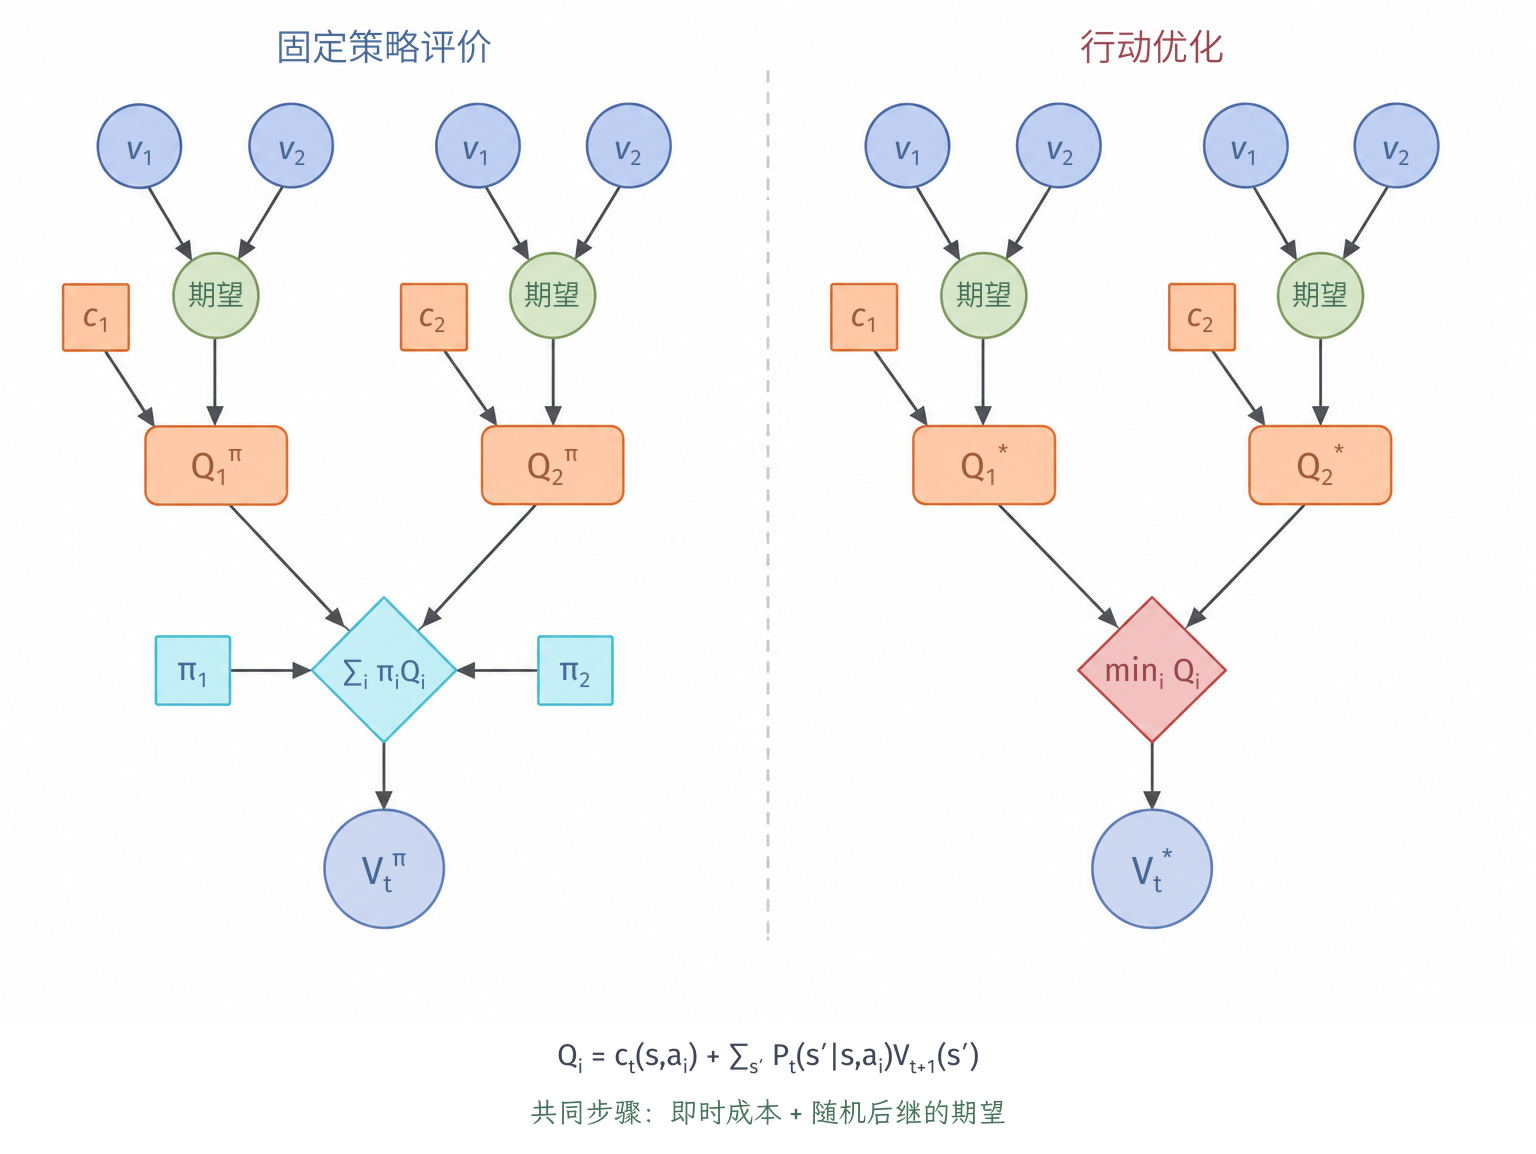
\includegraphics[width=\linewidth]{figures/01-mathematical-preliminaries/05-dynamical-systems-control-decision-and-games/generated/bellman-evaluation-versus-optimization/figure.png}
  \caption{成本口径下的两种Bellman递推。两边都先将即时成本与随机后继价值的期望相加；
  固定策略评价再按$\pi_t(a\mid s)$平均，最优递推则在允许行动之间取最小值，
  不能把行动最小化移到随机后继状态上。图中$c_i=c_t(s,a_i)$、$\pi_i=\pi_t(a_i\mid s)$；
  $v_1,v_2$是下一时刻两个后继状态的价值，左侧使用$V_{t+1}^\pi$，右侧使用$V_{t+1}^\star$，
  不暗示两边数值相同。有限时域边界为$V_H=c_H$，此处没有折扣系数。}
  \label{fig:bellman-evaluation-versus-optimization}
\end{figure*}


\begin{theorem}[有限时域最优性原理]
\label{thm:decision-finite-horizon-optimality}
在定义~\ref{def:decision-finite-mdp-policy}的有限MDP中，对每个末状态为$s$的历史
$h_t$，上述递推满足
$V_t^\star(s)=\inf_\pi J_t^\pi(h_t)$，其中下确界遍历全部允许的历史依赖随机继续策略。
各时刻各状态选择一个达到最小值的行动，构成达到该值的确定性Markov策略。
\end{theorem}
\begin{proof}
用逆向归纳。时刻$H$没有行动，终端成本就是最小继续成本。
假设每段末状态为$s'$的历史$h_{t+1}$的最小继续成本均为$V_{t+1}^\star(s')$。
固定末状态为$s$的$h_t$，任意策略先按$\pi_t(a\mid h_t)$选行动。
给定$a,s'$后，归纳假设说明其后续条件期望至少为$V_{t+1}^\star(s')$。
Markov转移保证下一状态分布是$P_t(\cdot\mid s,a)$，所以
\[
  J_t^\pi(h_t)\geq
  \sum_a\pi_t(a\mid h_t)
    \left[c_t(s,a)+\sum_{s'}P_t(s'\mid s,a)V_{t+1}^\star(s')\right]
  \geq V_t^\star(s).
\]
最后一步是有限个行动后果的凸组合不小于最小项。
反向在当前选择一个最小行动，并在每个下一状态采用归纳构造的最优Markov策略，
所有不等式均取等号。有限行动保证每次最小值达到，逆推到起点即得结论。
\end{proof}
证明比较了所有历史随机策略，不只比较Markov策略。Markov策略足够，是因为当前状态
概括了转移和期望累计目标所需信息；遗漏状态、整段轨迹的非加性指标或跨历史预算
都可能破坏这个前提。

\begin{example}[两阶段路线选择]
\label{ex:decision-two-stage-route}
回到前面固定的路线分布。终端价值就是终端损失，当前成本均为零，因而
\[
  Q_0(s_0,\text{稳妥})=2,\qquad
  Q_0(s_0,\text{捷径})=0.8\times0+0.2\times6=1.2.
\]
这里$Q_0$表示先指定当前行动、以后最优时的成本。期望准则应选择捷径，
而固定随机策略的成本$2-0.8p$也在$p=1$达到最小。
没有声称捷径每次都更好；它有概率$0.2$产生比稳妥更高的损失。
\end{example}

表~\ref{tab:decision-route-risk-criteria}保留同一轨迹模型，但改换评价口径。
风险偏好属于任务设定，不能在算完期望最优后将它解释成任意意义下的“最稳妥”。
\begin{table}[htbp]
  \centering
  \begin{tabular}{lcc}
    \toprule
    损失评价 & 稳妥 & 捷径\\
    \midrule
    $\mathbb E[L]$ & $2$ & $1.2$\\
    $P(L>3)$ & $0$ & $0.2$\\
    $\operatorname{VaR}_{0.9}(L)$ & $2$ & $6$\\
    $\operatorname{CVaR}_{0.9}(L)$ & $2$ & $6$\\
    \bottomrule
  \end{tabular}
  \caption{固定路线分布下的不同评价。捷径最坏$10\%$完全位于损失$6$的原子中，
  所以此处VaR与CVaR相同；这不是一般恒等式。增加违规概率预算后需重新选择策略。}
  \label{tab:decision-route-risk-criteria}
\end{table}

\subsubsection{无限折扣时域下的最优策略计算}

保留有限状态行动、时不变转移、有界成本及$0\leq\gamma<1$。与给定策略的
$T^\pi$不同，Bellman最优算子为
\begin{equation}
  (TV)(s)=\min_{a\in\mathcal A(s)}
    \left\{c(s,a)+\gamma\sum_{s'}P(s'\mid s,a)V(s')\right\}.
  \label{eq:decision-discounted-bellman-operator}
\end{equation}
对有限实数族$(u_a),(v_a)$，
$|\min_a u_a-\min_a v_a|\leq\max_a|u_a-v_a|$。
结合转移概率的非负性与归一化，得到
\begin{align}
  |(TV)(s)-(TW)(s)|
  &\leq\gamma\max_a
    \left|\sum_{s'}P(s'\mid s,a)(V(s')-W(s'))\right|\notag\\
  &\leq\gamma\lVert V-W\rVert_\infty,
  \label{eq:decision-bellman-contraction-pointwise}\\
  \lVert TV-TW\rVert_\infty&\leq\gamma\lVert V-W\rVert_\infty.
  \label{eq:decision-bellman-contraction}
\end{align}
有限维最大范数空间完备，定理~\ref{thm:analysis-banach-fixed-point}给出唯一固定点
$V^\star$。价值迭代$V^{(k+1)}=TV^{(k)}$从任意初值出发满足
\begin{equation}
  \lVert V^{(k)}-V^\star\rVert_\infty
  \leq\gamma^k\lVert V^{(0)}-V^\star\rVert_\infty.
  \label{eq:decision-value-iteration-error}
\end{equation}
固定点评价与最优性仍是两件事，必须证明该点由策略达到，并且不大于所有其他策略价值。

在每个状态选一个使$TV^\star(s)$取到最小值的行动，得到平稳确定策略$\pi^\star$。
此时$T^{\pi^\star}V^\star=TV^\star=V^\star$。固定策略评价算子的唯一固定点是
$V^{\pi^\star}$，由唯一性得$V^{\pi^\star}=V^\star$，所以候选值可实现。

再对任意历史依赖随机策略$\pi$比较。固定点满足每个状态行动的不等式
\[
  V^\star(s)\leq c(s,a)+\gamma\sum_{s'}P(s'\mid s,a)V^\star(s').
\]
沿策略实际选择的行动条件化，再把下一步的不等式代入，重复$n$步得到
\begin{equation}
  V^\star(s)\leq\mathbb E_s^\pi
  \left[\sum_{t=0}^{n-1}\gamma^tc(S_t,A_t)+\gamma^nV^\star(S_n)\right].
  \label{eq:decision-discounted-all-policy-comparison}
\end{equation}
该操作不要求$\pi$平稳，因为每一历史选择的行动都满足同一Bellman不等式。
余项绝对值至多$\gamma^n\lVert V^\star\rVert_\infty$，趋于零；
有界成本保证折扣级数可积。令$n\to\infty$得到$V^\star(s)\leq V^\pi(s)$。
与可达到性合起来，$\pi^\star$对全部允许历史随机策略最优。

若$\gamma=1$，严格压缩和尾项消失不再自动成立。长期平均成本
\[
  \limsup_{T\to\infty}\frac1T
    \mathbb E^\pi\left[\sum_{t=0}^{T-1}c(S_t,A_t)\right]
\]
采用了不同的目标：它衡量长期每步的成本，不是令折扣系数为$1$后直接累加全部成本。
要用同一个标量描述各初态的长期最优平均，需控制策略诱导链的常返结构。
有限模型的一种常见假设是：每项平稳确定性策略诱导的链都只有一个封闭常返类，
允许其余状态在进入该类之前被访问。这称为单链（unichain）假设；
它不要求只有一个状态，也不要求所有策略产生同一个转移矩阵。
在有限状态行动的单链模型中，平均成本最优性方程可写为
\[
  g+h(s)=\min_a\left\{c(s,a)+\sum_{s'}P(s'\mid s,a)h(s')\right\}.
\]
其中$g$是最优的长期每步平均成本，相对价值（relative value）$h(s)$记录从不同状态出发时，
相对于这个平均基线的成本偏移。对达到右侧最小值的平稳策略，逐步求和给出
\[
 \mathbb E_s\sum_{t=0}^{n-1}c(S_t,A_t)
 =ng+h(s)-\mathbb E_s h(S_n).
\]
这说明$ng$负责随时间增长的主项，$h$负责起点与终点的修正；有限状态下有界的修正除以$n$后消失。
方程的存在性属于平均成本理论，不能由前面的折扣压缩证明直接推出\scite{math-puterman1994mdp}

例如没有行动选择，两状态$s_0,s_1$确定性交替，阶段成本分别为$0,2$。
长期平均为$g=1$；取$h(s_0)=0,h(s_1)=1$，两状态的方程分别为
$1=0+1$与$2=2+0$。无折扣累计成本随时间发散，$h$却只记录状态之间的有限偏移。
给$h$加任意常数仍满足同一方程，可以约定参考状态$h(s_{\mathrm{ref}})=0$
消除这一自由度；这不等于已有折扣固定点的唯一性证明仍然适用。

连续状态或行动中，还需可测转移、适当的成本下半连续性、非空可行动作及紧致性或
强制性条件，再用可测选择将点态最小行动拼成策略。部分观测时只能使用允许信息；
信念状态只有在充分概括历史时才能承担这一角色。形式上写出$\inf$不等于它可达到。

\subsubsection{基于价值界与占用流量的最优性验证}

Bellman不等式给出一个有用的验证办法：提出一组状态价值下界，检查它对所有行动都成立。
与其对偶的是策略访问各状态行动对的折扣频率。给定初始分布$\mu_0$，价值端LP为
\begin{equation}
  \begin{aligned}
    \max_V\quad &(1-\gamma)\sum_s\mu_0(s)V(s)\\
    \text{s.t.}\quad&
      V(s)\leq c(s,a)+\gamma\sum_{s'}P(s'\mid s,a)V(s'),
      \quad s\in\mathcal S,\ a\in\mathcal A(s).
  \end{aligned}
  \label{eq:decision-value-lp}
\end{equation}
任意可行$V$满足$V\leq TV$，算子单调使
$V\leq TV\leq T^2V\leq\cdots$。令迭代收敛得到$V\leq V^\star$；
$V^\star$自身可行，因而达到最优值。
若$\mu_0$不在所有状态上为正，LP最优解未必唯一，但逐状态最大的可行向量仍是$V^\star$。

为每条不等式引入$d(s,a)\geq0$。最大化原问题的拉格朗日函数为
\[
  \begin{aligned}
    \mathcal L(V,d)&=(1-\gamma)\sum_s\mu_0(s)V(s)\\
    &\quad-\sum_{s,a}d(s,a)
      \left[V(s)-c(s,a)-\gamma\sum_{s'}P(s'\mid s,a)V(s')\right].
  \end{aligned}
\]
由于$V$自由取实值，$\sup_V\mathcal L(V,d)$有限当且仅当每个$V(s)$的系数为零，
即
\begin{equation}
  \sum_a d(s,a)=(1-\gamma)\mu_0(s)
    +\gamma\sum_{\bar s,\bar a}
      P(s\mid\bar s,\bar a)d(\bar s,\bar a).
  \label{eq:decision-discounted-flow-conservation}
\end{equation}
余下常数项为$\sum_{s,a}d(s,a)c(s,a)$，得到对偶
\begin{equation}
  \begin{aligned}
    \min_d\quad&\sum_{s,a}d(s,a)c(s,a)\\
    \text{s.t.}\quad&
      \text{式~\eqref{eq:decision-discounted-flow-conservation}},\qquad d(s,a)\geq0.
  \end{aligned}
  \label{eq:decision-occupancy-lp}
\end{equation}
原LP可行且有有限最优值，对偶也由下述任一策略产生可行点，
故有限LP强对偶定理~\ref{thm:opt-lp-strong-duality}给出两端最优值相等。

\begin{definition}[归一化折扣占用度量]
\label{def:decision-discounted-occupancy}
给定初始分布$\mu_0$、$0\leq\gamma<1$和允许策略$\pi$，归一化折扣
\term{占用度量}（occupancy measure）为
\begin{equation}
  d_\pi(s,a)=(1-\gamma)\mathbb E_{S_0\sim\mu_0}^\pi
    \left[\sum_{t=0}^\infty\gamma^t
      \mathbb I\{S_t=s,A_t=a\}\right].
  \label{eq:decision-discounted-occupancy}
\end{equation}
\end{definition}
它把同一状态行动在不同时刻的访问概率折扣相加，总质量为$1$，
通常不是Markov链的平稳分布。一般历史策略也有这样的占用。
分离$t=0$并将剩余时间索引前移，得到
\begin{align*}
  \sum_a d_\pi(s,a)
  &=(1-\gamma)\sum_{t=0}^\infty\gamma^t\mathbb P^\pi(S_t=s)\\
  &=(1-\gamma)\mu_0(s)
    +\gamma(1-\gamma)\sum_{t=0}^\infty\gamma^t
      \sum_{\bar s,\bar a}
      \mathbb P^\pi(S_t=\bar s,A_t=\bar a)P(s\mid\bar s,\bar a)\\
  &=(1-\gamma)\mu_0(s)+\gamma\sum_{\bar s,\bar a}
      P(s\mid\bar s,\bar a)d_\pi(\bar s,\bar a).
\end{align*}
所以流量方程的两项正是起点注入和后续转移注入。对状态求和得
$\sum_{s,a}d_\pi(s,a)=(1-\gamma)+\gamma\sum_{s,a}d_\pi(s,a)$，
从而总质量为$1$。成本对应关系为
\begin{equation}
  \sum_{s,a}d_\pi(s,a)c(s,a)
  =(1-\gamma)\mathbb E_{S_0\sim\mu_0}^\pi
    \left[\sum_{t=0}^\infty\gamma^tc(S_t,A_t)\right].
  \label{eq:decision-occupancy-cost}
\end{equation}

反过来，任一可行非负流量$d$也能实现。令$x_d(s)=\sum_a d(s,a)$，
在$x_d(s)>0$处定义$\pi_d(a\mid s)=d(s,a)/x_d(s)$，
零占用状态任意选行动。记相应转移矩阵为$\bm P_{\pi_d}$，状态占用列向量为$\bm x_d$，
则流量方程为
\[
  \bm x_d=(1-\gamma)\bm\mu_0+\gamma\bm P_{\pi_d}^{\top}\bm x_d.
\]
$\bm P_{\pi_d}$为行随机矩阵，$\bm I-\gamma\bm P_{\pi_d}^{\top}$的Neumann级数收敛，
因为$\lVert\gamma\bm P_{\pi_d}^{\top}\rVert_1=\gamma<1$。
所以此方程唯一可解。实际执行$\pi_d$所产生的状态占用满足同一方程，
必等于$\bm x_d$；再乘$\pi_d(a\mid s)$即恢复原来的$d(s,a)$。
因此对偶变量不是虚构的频率，而是可实施平稳随机策略的真实折扣访问分布。

互补松弛给出
\[
  d^\star(s,a)>0\ \Longrightarrow\
  V^\star(s)=c(s,a)+\gamma\sum_{s'}P(s'\mid s,a)V^\star(s').
\]
最优访问中实际使用的行动必须达到Bellman最小值。若不乘归一化因子$1-\gamma$，
流量方程起点项应为$\mu_0$，总质量为$1/(1-\gamma)$，目标也须同步改变。
连续状态下，占用成为测度、价值约束成为函数不等式；可测选择、紧致性和闭性等条件
仍需另证，不能只将求和改成积分便宣称强对偶成立。

\subsubsection{线性二次成本下的有限时域策略}

有限MDP通过逐行动枚举求最小值，线性二次模型则能利用代数结构直接求出最小行动。
前章定义~\ref{def:control-finite-horizon-lqr}已经给出有限时域LQR的问题，
定理~\ref{thm:control-finite-horizon-lqr}完整建立了Riccati递推及最优反馈。
本节只把这个结果接到本章的策略价值接口，不重复定义或配方证明。

该模型的最优继续价值具有
$V_t^\star(\bm x)=\bm x^\top\bm P_t\bm x+\beta_t$的形式。
式~\eqref{eq:control-lqr-bellman}是本节Bellman原理在连续线性状态上的具体版本：
线性动态代入下一步二次价值，仍得到关于当前状态和行动的二次函数；
前章通过严格正定的行动二次项求得
式~\eqref{eq:control-lqr-gain}的反馈增益，并由
式~\eqref{eq:control-discrete-riccati-recursion}反向计算$\bm P_t$。
零均值独立加性噪声的影响计入
式~\eqref{eq:control-lqr-noise-constant}的价值常数，不应在计算期望成本时丢弃。

给定反馈的评价只需代入该反馈；求最优反馈才需要对二次行动项最小化。
有限时域的最优性来自剩余成本的完整比较，不能推出无限时域闭环稳定；
后者使用前章定理~\ref{thm:control-infinite-horizon-lqr}的稳定化条件。
共同温度例的总输入成本也提醒我们，换成偏移输入$(u-0.4)^2$会改变目标。
若使用偏差坐标，应将原成本中的常数项和一次项一并变换，不能只套一个零目标LQR公式。

\subsection{连续演化下的策略优化}
\label{sec:control-hjb}

连续时间仍使用“当前一段成本加剩余最优价值”的原理，只是这一段可以任意短。
缩短时间间隔后，确定性速度产生价值的一阶导数，扩散噪声留下二阶导数。
方程给出局部关系，验证定理再把它与整段轨迹的最优性连接起来。

\subsubsection{确定性轨迹的价值方程}

考虑从$(\bm x,t)$出发的受控系统与成本
\begin{align}
  \dot{\bm x}(s)&=\bm f(\bm x(s),\bm u(s),s),\qquad \bm x(t)=\bm x,
  \label{eq:control-continuous-dynamics}\\
  J_{t,\bm x}(\bm u)
  &=\phi(\bm x(T))+\int_t^T\ell(\bm x(s),\bm u(s),s)\,\mathrm ds.
  \label{eq:control-continuous-cost}
\end{align}
状态属于$\mathbb R^n$，动作属于非空集合$U$。允许控制须可测、满足动作及状态约束，
并使轨迹在所考察时段存在、成本有限；反馈还须可由已有信息实现。
例如局部Lipschitz动态和适当增长界可用于保证常微分方程的适定性，
但写出一个不连续反馈后仍需重新核验。定义最优价值
$V(\bm x,t)=\inf_{\bm u}J_{t,\bm x}(\bm u)$。

若控制类对截断和前后拼接封闭，且具有所需近似最优选择，动态规划关系为
\begin{equation}
  V(\bm x,t)=\inf_{\bm u|_{[t,t+\Delta]}}
  \left\{\int_t^{t+\Delta}\ell(\bm x(s),\bm u(s),s)\,\mathrm ds
    +V(\bm x(t+\Delta),t+\Delta)\right\}.
  \label{eq:control-continuous-dpp}
\end{equation}
理由分为两边：任意全程控制的后半段成本不小于到达状态的最优继续价值，
所以全程下确界不小于右侧；反之将近似最优的短段与到达状态的近似最优继续控制拼接，
再使误差趋零，给出反向不等式。一般状态空间必须保证这些继续选择可测，
不能只对每条路径分别宣称存在一个后续控制。

经典方程的推导另假设$V\in C^1$、动态规划成立，且$\bm f,\ell$的连续性使短时
轨迹偏移为$O(\Delta)$。对参与逼近的控制还要求下面余项局部一致；
紧致动作集与相应局部有界连续系数是常见的充分条件。
以下在无状态约束的空间或约束不活跃的内部推导，保证所用常值动作在足够短的区间可行；
约束边界需另配边界条件。先用任意常值动作$\bm u$，
\begin{align*}
  V(\bm x(t+\Delta),t+\Delta)
  &=V(\bm x,t)+\Delta\,\partial_tV(\bm x,t)\\
  &\quad+\Delta\,\nabla_{\bm x}V(\bm x,t)^\top\bm f(\bm x,\bm u,t)
    +o(\Delta),\\
  \int_t^{t+\Delta}\ell(\bm x(s),\bm u,s)\,\mathrm ds
  &=\Delta\,\ell(\bm x,\bm u,t)+o(\Delta).
\end{align*}
用该控制代入下确界，只能先得到
\[
  -\partial_tV(\bm x,t)
  \leq\ell(\bm x,\bm u,t)+\nabla_{\bm x}V(\bm x,t)^\top\bm f(\bm x,\bm u,t).
\]
它对所有$\bm u\in U$成立，所以左侧不超过右侧的动作下确界。
要得到等式，还需要另一个方向，而不能把“任意动作”直接改写成“最优动作”。

固定$\eta>0$，取短段目标距下确界不超过$\eta\Delta$的允许控制。
沿轨迹使用链式法则，短段成本与价值增量等于
$\int_t^{t+\Delta}(\ell+\partial_sV+\nabla V^\top\bm f)\,\mathrm ds$。
一致余项允许把状态与时间冻结在$(\bm x,t)$；每个瞬时动作的Hamilton量均不低于
其动作下确界，于是
\[
  \partial_tV(\bm x,t)+
  \inf_{\bm u\in U}\{\ell(\bm x,\bm u,t)+
    \nabla_{\bm x}V(\bm x,t)^\top\bm f(\bm x,\bm u,t)\}
  \leq\eta+o(1).
\]
先令$\Delta\downarrow0$、再令$\eta\downarrow0$，与前一方向合并得到
\term{Hamilton--Jacobi--Bellman方程}（HJB）：
\begin{equation}
  -\partial_tV(\bm x,t)=
  \inf_{\bm u\in U}
    \{\ell(\bm x,\bm u,t)+
      \nabla_{\bm x}V(\bm x,t)^\top\bm f(\bm x,\bm u,t)\},
  \qquad V(\bm x,T)=\phi(\bm x).
  \label{eq:control-deterministic-hjb}
\end{equation}
花括号中的Hamilton量把瞬时成本和沿当前速度的价值变化率相加，
不是动力系统中沿轨迹守恒的Hamilton能量函数。
成本最小化对应这里的$\inf$和$-\partial_tV$；收益最大化须同步改换符号
\scite{math-bardi1997hjb}

\begin{theorem}[确定性HJB验证定理]
\label{thm:control-hjb-verification}
设候选$V\in C^1$满足式~\eqref{eq:control-deterministic-hjb}及终端条件。
假设每个允许控制都产生存在到$T$的轨迹，沿轨迹的链式法则和成本积分成立。
若有可实现反馈$\bm u^\star=\kappa(\bm x,t)$逐点达到HJB下确界，
且闭环轨迹存在到$T$并满足所有可行条件，则$V$为最优价值，$\kappa$为最优反馈。
\end{theorem}
\begin{proof}
任取允许控制，HJB的下确界不大于代入该动作的值，所以沿轨迹
\[
  \partial_sV(\bm x(s),s)+
  \nabla_{\bm x}V(\bm x(s),s)^\top
    \bm f(\bm x(s),\bm u(s),s)
  +\ell(\bm x(s),\bm u(s),s)\geq0.
\]
前两项由链式法则合为$\mathrm dV(\bm x(s),s)/\mathrm ds$。
从$t$积分到$T$，用终端条件得到$J_{t,\bm x}(\bm u)\geq V(\bm x,t)$。
因而候选值是所有允许成本的共同下界。
对$\kappa$，逐点达到下确界使不等式处处取等号，
积分后$J_{t,\bm x}(\kappa)=V(\bm x,t)$，所以它达到共同下界，完成验证。
\end{proof}
HJB是光滑最优价值满足的局部关系；验证定理则把一个候选解变成全程最优性的证书。
只在若干采样点降低方程残差还不够，还需终端或边界条件、极小动作的可实现性、
轨迹存在性及整个相关区域上的方程关系。

\subsubsection{随机轨迹的价值方程}

随机轨迹无法逐条预先选择，但可以优化允许策略的期望成本。设$\bm W_s$为
$d$维标准Brownian运动，状态满足
\begin{equation}
  \mathrm d\bm X_s=\bm f(\bm X_s,\bm u_s,s)\,\mathrm ds
    +\bm\Sigma(\bm X_s,\bm u_s,s)\,\mathrm d\bm W_s,
  \label{eq:control-stochastic-dynamics}
\end{equation}
其中$\bm\Sigma$为$n\times d$矩阵。允许控制对给定滤过渐进可测，
不得使用未来Brownian增量，并满足解存在、约束与成本可积的要求。
价值为
$\inf_{\bm u}\mathbb E_{t,\bm x}[
\phi(\bm X_T)+\int_t^T\ell(\bm X_s,\bm u_s,s)\,\mathrm ds]$；
下标表示从$(t,\bm x)$重启过程，避免对零概率初态事件直接作比值条件化。

对$V\in C^{2,1}$应用第~\ref{chap:dynamical-systems-and-state-estimation}章的
Itô公式，固定动作的受控生成元为
\[
  \mathcal L^{\bm u}V=
  \nabla_{\bm x}V^\top\bm f+
  \frac12\operatorname{tr}
    (\bm\Sigma\bm\Sigma^\top\nabla_{\bm x}^2V).
\]
随机积分在可积鞅条件下的条件均值为零，二次变差却留下了二阶项。
在动态规划、近似最优选择及局部一致的短时展开条件下，先代入常值动作得到一个方向，
再沿$\eta\Delta$-最优控制积分并令$\Delta,\eta$趋零，得到
\begin{equation}
  \begin{aligned}
  -\partial_tV(\bm x,t)=\inf_{\bm u\in U}\biggl\{&
    \ell(\bm x,\bm u,t)+
    \nabla_{\bm x}V(\bm x,t)^\top\bm f(\bm x,\bm u,t)\\
    &+\frac12\operatorname{tr}\!\left[
      \bm\Sigma(\bm x,\bm u,t)\bm\Sigma(\bm x,\bm u,t)^\top
      \nabla_{\bm x}^2V(\bm x,t)\right]\biggr\}.
  \end{aligned}
  \label{eq:control-stochastic-hjb}
\end{equation}
终端条件仍为$V(\bm x,T)=\phi(\bm x)$。这里对随机微分方程仅取均值后代入
确定性HJB，会遗漏扩散项。

\begin{theorem}[随机HJB验证]
\label{thm:control-stochastic-hjb-verification}
设$V$对状态二次、对时间一次连续可微，满足
式~\eqref{eq:control-stochastic-hjb}及终端条件。
假设每个允许控制都使受控过程存在到$T$，成本与Itô公式中的有限变差项可积，
且$\int_t^s\nabla_{\bm x}V^\top\bm\Sigma\,\mathrm d\bm W$为真鞅。
若可容许反馈$\bm u^\star=\kappa(\bm x,t)$逐点达到HJB下确界，
则$V$等于最优期望成本，$\kappa$达到该值。
\end{theorem}
\begin{proof}
对任意允许控制，HJB给出
$\partial_sV+\mathcal L^{\bm u_s}V+\ell(\bm X_s,\bm u_s,s)\geq0$。
沿轨迹应用Itô公式、积分并取从$(t,\bm x)$出发的期望，随机积分因真鞅条件消失，
得到
\[
  \mathbb E_{t,\bm x}\left[
    \phi(\bm X_T)+\int_t^T\ell(\bm X_s,\bm u_s,s)\,\mathrm ds\right]
  \geq V(\bm x,t).
\]
对$\kappa$，生成元不等式取等号，同一计算证明其期望成本等于共同下界$V$。
这验证的是期望最优，不是每条噪声实现上的路径最优。
\end{proof}

一个常用的充分鞅条件是
$\mathbb E\int_t^T\lVert\bm\Sigma^\top\nabla_{\bm x}V\rVert^2\,\mathrm ds<\infty$。
若只能得到局部鞅，应先在退出有界区域等停时$\tau_n$处停止，再证明成本积分、
$V(\bm X_{T\wedge\tau_n},T\wedge\tau_n)$等量能合法取极限，例如使用增长界、
矩估计与一致可积性。局部鞅不自动具有零期望，省略这一步会使验证结论失去依据。

若扩散矩阵与状态、动作都无关，二次价值的二阶项只增加状态无关的常数，
对应离散式~\eqref{eq:control-lqr-noise-constant}的现象。
若扩散依赖动作，它直接参与动作最小化；依赖状态时也可能改变价值形状。
因此噪声均值为零并不足以保证反馈不变。

\subsubsection{线性二次成本下的连续策略}

在线性动态$\dot{\bm x}=\bm A\bm x+\bm B\bm u$下，
取$\bm u\in\mathbb R^m$，阶段成本
$\ell(\bm x,\bm u)=\bm x^\top\bm Q\bm x+\bm u^\top\bm R\bm u$，
终端成本$\phi(\bm x)=\bm x^\top\bm Q_T\bm x$，其中
$\bm Q,\bm Q_T\succeq\bm0$、$\bm R\succ\bm0$。有限时域取平方可积控制，
固定有限矩阵保证线性轨迹存在。试取对称二次候选
\[
  V(\bm x,t)=\bm x^\top\bm P(t)\bm x,\qquad \bm P(T)=\bm Q_T.
\]
它是否确为价值要由HJB和验证定理确认，而不是由二次外形决定。
有
$\partial_tV=\bm x^\top\dot{\bm P}\bm x$、
$\nabla_{\bm x}V=2\bm P\bm x$。代入HJB后动作相关项为
$\bm u^\top\bm R\bm u+2\bm x^\top\bm P\bm B\bm u$，配方得
\begin{align*}
  \bm u^\top\bm R\bm u+2\bm x^\top\bm P\bm B\bm u
  ={}&
  (\bm u+\bm R^{-1}\bm B^\top\bm P\bm x)^\top
    \bm R(\bm u+\bm R^{-1}\bm B^\top\bm P\bm x)\\
  &-\bm x^\top\bm P\bm B\bm R^{-1}\bm B^\top\bm P\bm x.
\end{align*}
正定$\bm R$使第一项非负且仅在一个动作处为零，因此反馈为
\begin{equation}
  \bm u^\star(t)=-\bm R^{-1}\bm B^\top\bm P(t)\bm x(t).
  \label{eq:control-continuous-lqr-gain}
\end{equation}
把最小项代回，对所有$\bm x$比较二次型系数，得到
\begin{equation}
  -\dot{\bm P}
  =\bm Q+\bm A^\top\bm P+\bm P\bm A
    -\bm P\bm B\bm R^{-1}\bm B^\top\bm P,\qquad
  \bm P(T)=\bm Q_T.
  \label{eq:control-continuous-riccati}
\end{equation}
这是微分Riccati方程；价值边界给在终点，故从$T$向较早时刻反向积分。

有限时域上这些条件也保证不会在中途丢失所需解。矩阵常微分方程先在终端附近有唯一
局部对称解；在其存在区间，反馈连续，验证定理说明其二次型为非负最优成本，
并不大于零控制的有限成本。零控制在整个有限区间给出统一的二次上界，
于是$\bm0\preceq\bm P(t)\preceq M\bm I$，某个有限$M$适用于该区间。
局部Lipschitz的Riccati向量场因解有界而可继续延伸，直到起点。
因此该候选及反馈确实定义在整个有限时域。

还可以直接给出成本差证书。用Riccati方程化简沿任意允许轨迹的价值导数，得到
\[
  \ell(\bm x,\bm u)+\frac{\mathrm d}{\mathrm dt}
    [\bm x^\top\bm P(t)\bm x]
  =
  (\bm u+\bm R^{-1}\bm B^\top\bm P\bm x)^\top
    \bm R(\bm u+\bm R^{-1}\bm B^\top\bm P\bm x).
\]
积分后，任意策略的成本等于初始二次价值加右侧非负积分；
反馈使积分为零，最优性由此可以逐项核算。
例如$\dot x=u$、$Q=R=1,Q_T=0$时，
$P(t)=\tanh(T-t)$满足$-\dot P=1-P^2$，
反馈$u=-\tanh(T-t)x$，价值为$\tanh(T-t)x^2$。
越接近没有终端惩罚的截止时刻，控制增益越小，这也说明有限时域策略一般依赖时间。

无限时域的代数方程与稳定化条件由前章式~\eqref{eq:control-care}给出，
这里不把令$\dot{\bm P}=0$当作稳定性证明。
连续闭环需要特征值实部为负，离散闭环需要特征值位于单位圆内；
CARE与DARE分别服务于这两个问题，不能混用。

\subsubsection{非光滑与受限信息下的价值方程}

最优动作切换时，价值可能连续但没有处处存在的梯度。
经典HJB在折点不能直接代入，这不表示轨迹成本没有定义。
\term{黏性解}（viscosity solution）用光滑函数从上方或下方接触价值，
在接触点检验方程不等式；导数取自测试函数，价值本身可以不可微。

将确定性HJB写成
\[
  F(\bm x,t,a,\bm p)
  :=-a-\inf_{\bm u\in U}
      \{\ell(\bm x,\bm u,t)+\bm p^\top\bm f(\bm x,\bm u,t)\}=0,
\]
其中$a$代表时间导数，$\bm p$代表状态梯度。
\begin{definition}[连续价值函数的黏性解]
\label{def:control-viscosity-solution}
设$V$在方程作用域内连续。对任意光滑测试函数$\varphi$，
若$V-\varphi$在内点$(\bm x,t)$取局部最大值时均有
$F(\bm x,t,\partial_t\varphi,\nabla_{\bm x}\varphi)\leq0$，
称$V$为黏性次解。若局部最小值处均有相应的$F\geq0$，称为黏性上解。
同时满足两项，并按当前问题满足终端或边界条件的$V$称为黏性解。
\end{definition}
可将测试函数平移常数使接触时$V=\varphi$。
局部最大对应$\varphi$从上方接触，局部最小对应从下方接触；
不是任取一个斜率代入。随机二阶方程还需代入测试函数的Hessian。
光滑$V$取$\varphi=V$即恢复经典等式。适当的比较原理可由次解不高于上解推出唯一性，
但其方程结构、连续性、增长与边界条件仍需另证，定义本身不保证唯一或易于计算。

先看目标边界上的非光滑。令$\dot x=u,|u|\leq1$，每单位时间成本为$1$，
到达$\{0\}$即终止，则最短到达时间$V(x)=|x|$。在延续域$x\neq0$上，
\[
  0=1+\inf_{|u|\leq1}V'(x)u=1-|V'(x)|.
\]
正侧取$u=-1$、负侧取$u=1$，均推向原点。$x=0$是退出边界，
只需施加$V(0)=0$，不属于方程内部。这个例子不能单独证明内点必须使用黏性解；
要展示内点折角，需要一个不在原点提前退出的问题。

\begin{example}[延续域内部的价值折点]
\label{ex:control-viscosity-interior-kink}
仍取$\dot x=u,|u|\leq1$，改为固定终点$T$、零运行成本和终端成本$|x(T)|$。
剩余时间最多移动$T-t$，故
\[
  V(x,t)=\max\{|x|-(T-t),0\},\qquad
  -V_t+|V_x|=0,\qquad V(x,T)=|x|.
\]
内侧$|x|<T-t$可以到达原点并停留，价值为零；外侧只能减少$T-t$的距离。
折点$x=\pm(T-t)$位于$t<T$的延续域内部。例如$T-t=1$时，
$|x|\leq1$可完全纠正，$x=1.5$仍剩终端代价$0.5$。

正侧折点附近$V=\max\{x+t-T,0\}$。从下方接触的光滑函数的导数对
$(\varphi_x,\varphi_t)$为$(p,p)$、$0\leq p\leq1$，
即两侧斜率的凸组合，故$-\varphi_t+|\varphi_x|=-p+p=0$，满足上解条件。
向上折角不存在光滑上方接触函数，次解检验在该点无额外约束；
光滑区域满足经典等式。负侧接触导数为$(-p,p)$，同样满足等式。
这说明黏性条件能处理方程内部的切换折点，而不把切换面误当作退出边界。
\end{example}

有状态约束时，价值只在可行控制存在的区域定义。不可穿越边界需配合可行方向
或状态约束边界条件；允许触边退出则需退出成本。内部方程相同不能代替边界含义。
真实状态不可见时，也不能直接以$\bm x$作为反馈输入，一般须使用观测历史给出的
\term{信念状态}，通常是无限维分布。线性高斯二次模型的有限维分离是特殊结构，
将在下一节证明其成本最优性。

HJB比较累计成本，前章的屏障约束限定安全行动。将屏障二次规划用于修正一个性能反馈，
通常会改变原成本最优性；在HJB中直接加入约束则是另一个受约束优化问题。
稳定性证明使用的Lyapunov函数、最优价值和屏障函数分别服务于收敛、最优与不变性，
不能仅因它们都考察沿轨迹的标量变化而互换。

\subsection{受限信息下的策略选择}
\label{sec:decision-value-of-information}

\subsubsection{新增观测下的决策收益}

前面的最优规则都受到已有信息限制。如果先获得一次观测，后面的行动可能随观测改变，
这项改进能否抵偿获取成本？答案依赖任务损失，不只依赖观测减少了多少不确定性。
设未知环境参数为$\Theta$、当前信息为$\mathcal G$，信念为
$b(\mathrm d\theta)=\mathbb P(\Theta\in\mathrm d\theta\mid\mathcal G)$。
先取有限行动与可测可积损失；立即行动的最小风险为
\[
  \mathcal R(b)=\inf_a\mathbb E_{\theta\sim b}[\ell(a,\theta)].
\]
现在可先从给定核$K(\mathrm dz\mid\theta)$观察信号$Z$，得到后验$b_Z$，
再选适合该后验的行动。

\begin{definition}[期望样本信息价值]
\label{def:decision-expected-sample-information-value}
在上述有限行动、可积损失和信号核条件下，\term{期望样本信息价值}
（expected value of sample information, EVSI）为
\begin{equation}
  \operatorname{EVSI}(Z\mid b)
  =\mathcal R(b)-\mathbb E_{Z\mid b}[\mathcal R(b_Z)].
  \label{eq:decision-evsi}
\end{equation}
\end{definition}
观察后的$\inf_a$在对$Z$求期望之内：先见信号、再行动。
若把$\inf_a$放在外面，就强迫所有信号结果使用同一行动，丢失信息的用途。
这比较的是两种信息条件下的最优值，不是同一固定策略多观测一次后的数值变化。

EVSI非负，因为看到信号后总可忽略它。若原最优行动为$a^\star$，则
\[
  \mathcal R(b_z)\leq
  \mathbb E[\ell(a^\star,\Theta)\mid Z=z,\mathcal G].
\]
对$Z$平均并用塔式法则，得到
$\mathbb E_{Z\mid b}[\mathcal R(b_Z)]\leq
\mathbb E[\ell(a^\star,\Theta)\mid\mathcal G]=\mathcal R(b)$。
一般行动空间若下确界不达到，可用风险至多$\mathcal R(b)+\varepsilon$的行动，
作同样比较后令$\varepsilon\downarrow0$；但观察后的选择还须具有可测的
最优或近似最优规则。免费信息不降低最优收益，不意味着有成本的信息都值得购买：
获取成本为$k$时，净价值是$\operatorname{EVSI}-k$。

若直接知道$\Theta$，\term{完全信息价值}为
\begin{equation}
  \operatorname{EVPI}(b)
  =\inf_a\mathbb E_b[\ell(a,\Theta)]
    -\mathbb E_b[\inf_a\ell(a,\Theta)].
  \label{eq:decision-evpi}
\end{equation}
已知$\Theta$可模拟信号核，再执行任何基于信号的规则，
故$0\leq\operatorname{EVSI}\leq\operatorname{EVPI}$。
等号$\operatorname{EVSI}=\operatorname{EVPI}$表示信号已保留实现该任务最优行动所需的
信息，不要求重建参数的每个细节。

\begin{example}[辨别信号与无关信号]
\label{ex:decision-informative-and-irrelevant-signals}
阳性概率为$0.3$，假阳性损失为$1$、假阴性为$9$。
不取新信号时，两行动风险为$0.7$和$2.7$，所以$\mathcal R(b)=0.7$。
免费信号$Z_{\mathrm{perf}}$若完全揭示类别，观察后总能选对，
风险为零，EVSI为$0.7$。独立于类别的公平硬币$Z_{\mathrm{coin}}$不改变后验、
行动或风险，EVSI为零。若完全信号成本为$0.8$，其净价值为$-0.1$。
信息能否辨别类别、是否改善任务、是否抵偿获取成本，是三个不同判断。
\end{example}

互信息衡量关于$\Theta$的不确定性平均减少多少，EVSI衡量给定损失下最优决策改善多少。
信号可能精确揭示与行动无关的参数，互信息大而EVSI为零；另一个信号只在决策阈值附近
改变信念，却可能避免高代价行动。对数评分下，若行动本身是预测分布，最优期望对数损失
与条件熵对应，才得到信息增益与风险改善的直接联系。一般分类、分配和控制损失没有这种
自动等价；使用熵作为查询代理，需要额外论证它与任务成本的关系。

\subsubsection{未知收益下的探索价值}

信息不一定来自独立购买的信号，也可能来自行动自身的结果。
考虑两轮选择，每次成功奖励$1$、失败奖励$0$，本小节改用收益最大化，
对应成本为奖励的负值。已知臂的成功概率为$0.6$；
未知臂有一个两轮不变的参数$\Theta\in\{0.3,0.9\}$，先验各为$1/2$。
给定$\Theta$，各次奖励条件独立，已知臂结果不提供$\Theta$的信息。
每轮只看到所选臂结果，不看到未选臂的反事实结果。

两臂当前平均成功率均为$0.6$，只比第一轮即时收益会并列。
先选未知臂时，成功的边缘概率为$0.6$。看到成功后，
\[
  \mathbb P(\Theta=0.9\mid\text{成功})
  =\frac{0.9\times0.5}{0.9\times0.5+0.3\times0.5}=0.75,
\]
未知臂下一轮成功率为$0.75\times0.9+0.25\times0.3=0.75$，应继续选它。
若看到失败，
\[
  \mathbb P(\Theta=0.9\mid\text{失败})
  =\frac{0.1\times0.5}{0.1\times0.5+0.7\times0.5}=0.125,
\]
未知臂后验成功率为$0.125\times0.9+0.875\times0.3=0.375$，
下一轮应改选已知臂。因此两轮最优适应行动的期望收益为
\begin{equation}
  0.6+0.6\times0.75+0.4\times0.6=1.29.
  \label{eq:decision-two-arm-information-value}
\end{equation}
先选已知臂不会更新信念，第二轮仍并列，两轮收益为$1.2$。
多出的$0.09$来自第一轮观测改善第二轮选择，不来自未知臂的当前均值较高。

这就是\term{探索}（exploration）的决策作用：行动同时影响当前收益和未来信息。
只剩一轮时，信息没有使用机会，两臂又并列；试验成本、先验或剩余时域改变，
探索价值也会改变。若每轮同时看到所有臂，或$\Theta$随时间漂移，上述信息结构已不成立，
后验和$1.29$的计算也不再适用。一般多臂和强化学习算法还须处理长期规划、
未知参数与计算复杂度，这个两轮例子只定位信息价值从哪里进入策略。

自适应查询也改变统计证据的条件。因为过去观察决定下一次试验或停止时间，
不能把选中样本无条件视为固定设计下的独立同分布数据。
报告置信区间或最优行动识别保证时，应回用
第~\ref{sec:stoch-martingales-stopping-sequential-concentration}节的停时条件与
第~\ref{sec:stoch-self-normalized-adaptive-design}节的可预测设计，
检查行动是否在当前噪声揭晓前选定，以及误差保证是否对全部查看时刻同时成立。

遗憾使用另一个比较对象。令$Y_t$为第$t$轮奖励，
$\mathcal H_{t-1}$为行动前信息，行动$A_t$在$Y_t$揭晓前选定，
并假设对固定环境参数$\theta$，
\[
  \mathbb E[Y_t\mid\mathcal H_{t-1},A_t=a,\Theta=\theta]
  =\mu(a,\theta)\quad\text{几乎处处}.
\]
这里平均奖励不随轮次改变；条件均值假设使自适应选择后当前噪声仍正确中心化，
却不使访问次数或全部数据变成非自适应。令
$a^\star(\theta)\in\argmax_a\mu(a,\theta)$，累计伪遗憾为
\[
  \operatorname{Reg}_T(\theta)
  =\sum_{t=1}^T[\mu(a^\star(\theta),\theta)-\mu(A_t,\theta)].
\]
它比较同一环境下的平均奖励，而不是两条实现奖励轨迹之差。
算法和参数随机时还可再取期望；直接用实现奖励定义的遗憾含有奖励噪声。
一次信号的EVSI与长期伪遗憾相关，但前者不能替代后者的统计与序贯证明。

\subsubsection{线性高斯条件下的估计与行动分离}

一般情况下，行动改变未来信息，会像探索例那样同时影响估计和控制。
一个重要的例外是标准有限时域线性二次高斯控制（LQG）。
取
\[
  \bm x_{t+1}=\bm A\bm x_t+\bm B\bm u_t+\bm w_{t+1},
  \qquad \bm y_t=\bm C\bm x_t+\bm v_t,
\]
其中$\bm x_0$高斯，$\bm w_{t+1}\sim\mathcal N(\bm0,\bm W_t)$、
$\bm v_t\sim\mathcal N(\bm0,\bm N_t)$，$\bm W_t\succeq\bm0$、$\bm N_t\succ\bm0$，
初态与所有噪声相互独立，噪声跨时独立，协方差已知且不依赖控制。
先观察$\bm y_t$再行动，信息为
$\mathcal I_t=\sigma(\bm y_0,\bm u_0,\ldots,\bm u_{t-1},\bm y_t)$。
允许无输入或状态约束、具有有限二阶矩的$\mathcal I_t$-可测控制；
若使用私有随机数，也将独立于系统噪声的已用随机数计入可用信息。
目标为前章有限LQR的期望二次成本，状态和终端权重半正定、输入权重正定。

第~\ref{sec:dynamical-kalman-rts}节的有限时域Kalman递推给出
$\widehat{\bm x}_t=\mathbb E[\bm x_t\mid\mathcal I_t]$和更新后误差协方差
$\bm E_t=\mathbb E[(\bm x_t-\widehat{\bm x}_t)
(\bm x_t-\widehat{\bm x}_t)^\top\mid\mathcal I_t]$。
令$\bm e_t=\bm x_t-\widehat{\bm x}_t$，投影性质说明
$\mathbb E[\bm e_t\mid\mathcal I_t]=\bm0$，从而
\[
  \mathbb E[\bm x_t^\top\bm Q_t\bm x_t\mid\mathcal I_t]
  =\widehat{\bm x}_t^\top\bm Q_t\widehat{\bm x}_t
    +\operatorname{tr}(\bm Q_t\bm E_t).
\]
交叉项的条件期望为零，因而无条件也有
$\mathbb E[\widehat{\bm x}_t^\top\bm Q_t\bm e_t]=0$。
标准模型的关键在于$\bm E_t$由Kalman协方差递推确定，不依赖观测值或所选控制。
控制在预测均值中作为已知平移被扣除，不改变下一次观测的误差协方差。

只看这一项分解还不能证明全程最优，需要把所有未来动作的影响合在一起。
令$\bm P_t,\bm K_t$取前章有限LQR递推的结果，
$\bm M_t=\bm R_t+\bm B^\top\bm P_{t+1}\bm B\succ\bm0$。
回用前章逐步配方并对时间求和，任一允许输出策略$\mu$满足
\begin{align*}
  J^\mu={}&
    \mathbb E[\bm x_0^\top\bm P_0\bm x_0]
    +\sum_{t=0}^{H-1}\operatorname{tr}(\bm P_{t+1}\bm W_t)\\
    &+\sum_{t=0}^{H-1}\mathbb E[
      (\bm u_t+\bm K_t\bm x_t)^\top
      \bm M_t(\bm u_t+\bm K_t\bm x_t)].
\end{align*}
此式来自状态价值项的望远镜消去和独立零均值噪声的迹项，
不是假设输出策略已经最优。再对$\mathcal I_t$条件化，最后一项逐步分为
\begin{align*}
  &\mathbb E[
    (\bm u_t+\bm K_t\bm x_t)^\top\bm M_t
    (\bm u_t+\bm K_t\bm x_t)\mid\mathcal I_t]\\
  &\quad=
    (\bm u_t+\bm K_t\widehat{\bm x}_t)^\top\bm M_t
    (\bm u_t+\bm K_t\widehat{\bm x}_t)
    +\operatorname{tr}(\bm K_t^\top\bm M_t\bm K_t\bm E_t).
\end{align*}
所有迹项与初态项都不依赖策略。剩余各项非负，而可实施策略
\begin{equation}
  \bm u_t^\star=-\bm K_t\widehat{\bm x}_t
  \label{eq:policy-finite-lqg-feedback}
\end{equation}
使这些项同时为零，因而在全部允许输出策略中达到最小期望成本。
误差协方差产生的成本并未消失，只是不能通过该模型中的控制改变。

这就是\term{分离原则}：有限Kalman滤波按估计误差构造条件均值，
LQR增益按行动成本构造，再将二者连接。它比确定性观测器的谱分离多给出成本最优性，
却不要求有限时域滤波已经达到稳态；稳态滤波和输出反馈的稳定条件仍由前章负责。
受控观测、动作相关噪声、风险敏感目标、输入或状态约束会改变上述分解或可行性，
不能直接沿用这一结论。温度例中的有界两点噪声也不是这里的高斯假设；
若采用LQG模型，应显式另取独立高斯噪声，并放弃将有界安全区间视为逐路径必然保证。

\subsection{风险约束下的策略优化}
\label{sec:policy-risk-optimization}

现在把风险评价接口中的指定动作改成待选择动作。必须先固定目标：
嵌套条件风险可以按其定义逐步优化；静态总损失CVaR使用累计状态；
概率约束和候选模型又分别规定可行策略与最坏机制。它们并不是互换风险符号的同一个算法。

对有限状态行动、确定Markov策略和具有充分状态信息的嵌套风险，
单调性允许把每个下一状态的最优继续值用于当前比较：
\begin{align}
  V_H(s)&=c_H(s),\notag\\
  V_t(s)&=\min_{a\in\mathcal A(s)}
    \{c_t(s,a)+\rho_{t,s,a}(V_{t+1}(S_{t+1}))\}.
  \label{eq:decision-risk-bellman-finite}
\end{align}
有限时域的证明仍是逆向归纳，但将期望的保序性换成风险映射的单调性。
任一允许的历史依赖确定策略，其后续风险逐节点不低于$V_{t+1}$，
当前风险便不低于相应动作项；
取最小动作再接上各节点的最优继续策略达到此界。
这要求允许规则能逐历史拼接、风险模型在相同状态使用相同映射。
取条件期望恢复普通Bellman；取条件CVaR得到嵌套CVaR，而非静态CVaR
\scite{math-ruszczynski2010risk}

若允许随机行动并采用第~\ref{sec:policy-nested-risk-evaluation}节“先评价环境风险、
再平均行动风险”的口径，行动概率的目标为各动作项的线性组合，确定最小动作仍足够。
若声明风险作用于行动和下一状态的联合损失，则应优化概率分布$q\in\Delta(\mathcal A(s))$：
\[
  \inf_q\,\rho^q_{t,s}\bigl(c_t(s,A)+V_{t+1}(S')\bigr).
\]
不能无条件用期望的线性性把它写成动作风险的平均，再声称确定策略最优。
给定更具体的风险泛函可另证随机化是否有益；本节上式
~\eqref{eq:decision-risk-bellman-finite}的策略范围以已声明的口径为准。

无限折扣版本明确按“后续风险值再乘折扣”的目标定义算子
\begin{equation}
  (T_\rho V)(s)=\min_a
    \{c(s,a)+\gamma\rho_{s,a}(V(S'))\}.
  \label{eq:decision-risk-bellman-operator}
\end{equation}
成本有界、每个映射归一化、单调且平移等变时，
第~\ref{sec:policy-nested-risk-evaluation}节已证一步风险非扩张；
再用最小值差不等式得到
\begin{equation}
  \lVert T_\rho V-T_\rho W\rVert_\infty
  \leq\gamma\lVert V-W\rVert_\infty.
  \label{eq:decision-risk-bellman-contraction}
\end{equation}
因此$\gamma<1$时唯一固定点存在，价值迭代误差不超过
$\gamma^k\lVert V^{(0)}-V^\star_\rho\rVert_\infty$，
残差界为$\lVert T_\rho V-V\rVert_\infty/(1-\gamma)$。

最优解释还须补全。固定点的贪心策略使固定策略风险算子取同一个固定点，故达到该值。
有限截断问题用上述逆向归纳比较全部允许历史策略；若$|c|\leq C$，
归一化和非扩张使第$n$步以后的折扣风险影响至多为
$\gamma^nC/(1-\gamma)$，统一趋于零。因此截断最优值和各允许策略的截断值
可取极限，得到固定点不大于任何策略的无限嵌套风险。
如果原风险目标并非如此递归、状态遗漏历史信息或策略类不可拼接，
算子即使压缩，也只是稳定地计算另一个问题。

相干映射的包络把动作项改写成
\[
  c(s,a)+\gamma\sup_{q\in\mathcal Q(s,a)}
    \sum_{s'}q(s'\mid s,a)V(s').
\]
将它解释为逐时鲁棒最优，必须使用定义~\ref{def:decision-rectangular-uncertainty}
的矩形候选机制。共享未知参数的非矩形集合不能逐节点自由取最坏；
有限凸风险若有对偶罚项，也不能在优化时删去。

静态CVaR则回用第~\ref{sec:policy-static-cvar-evaluation}节的累计状态。
固定$\eta$，将式~\eqref{eq:policy-static-cvar-augmented-evaluation}中的行动概率汇总
改成行动最小化，得到
\[
  \begin{aligned}
    W_t^\eta(s,b)&=\min_a\sum_{s'}P_t(s'\mid s,a)
      W_{t+1}^\eta(s',b+\gamma^tc_t(s,a)),\\
    W_H^\eta(s,b)&=(b+\gamma^Hc_H(s)-\eta)_+.
  \end{aligned}
\]
随后计算
\[
  \inf_\pi\operatorname{CVaR}_\alpha(L^\pi)
  =\inf_{\eta\in\mathbb R}
    \left\{\eta+\frac{1}{1-\alpha}
      \sum_s\mu_0(s)W_0^\eta(s,0)\right\}.
\]
两层均为下确界，因此交换$\inf_\pi,\inf_\eta$不需要极小极大定理，
但须说明策略类：这里允许时间、物理状态和累计成本上的策略，
并假设可测选择与所需达到性。阈值是起点选定的常数，不能到未来看到损失后重新挑选。
若原问题只允许不读取累计成本的策略，这项动态规划可能扩大可行策略类；
若只存在下确界，可使用近似最优阈值和策略，不能宣称必有最优解。

概率约束问题例如
$\inf_{\pi:\,\mathbb P^\pi(E)\leq\varepsilon}\mathbb E^\pi[L]$
限制的是特定违规事件$E$。终端、逐时和全程事件须分别定义；
全程约束可能需要增广累计违规标记或剩余风险预算。
路线例要求$\mathbb P^\pi(L>3)\leq0.1$时，随机策略须满足$0.2p\leq0.1$，
即$p\leq1/2$。期望损失$2-0.8p$在$p=1/2$取$1.6$；
若只允许确定行动，则只有稳妥可行，成本$2$。随机化的作用来自概率约束的可行比例，
不能用无约束纯策略最优结论排除它。

最坏模型目标为
\[
  \inf_{\pi\in\Pi_{\mathrm{adm}}}
    \sup_{Q\in\mathcal P}\mathbb E_Q^\pi[L].
\]
单步时退化为$\inf_a\sup_Q\mathbb E_Q[\ell(a,Y)]$，参数模型用$Q=P_\theta$。
$\Pi_{\mathrm{adm}}$须规定信息和约束，$\mathcal P$须规定模型能否随历史改变。
对偶、极小极大交换和局部递推分别有自己的条件。
评价准则、时间一致性、可行性与计算收敛各回答一项问题，不能用其中一个替代其他检查。

\section{本章小结}
\label{sec:decision-theory-and-dynamic-risk-summary}

同一两阶段路线任务串起了本章四个步骤。策略先规定走捷径的概率$p$，
再与环境共同产生概率为$1-p,0.8p,0.2p$的三条轨迹；给每条轨迹计价后，
期望损失为$2-0.8p$，尾部指标和违规概率还描述它的其他后果。
固定$p$计算这些量是评价，允许改变$p$才是优化。期望准则选$p=1$，
概率预算可能要求$p\leq1/2$，因此“最优”离不开准则和可行域。

平均收益、一次实现收益和尾部损失不是同一个对象。VaR给出分位阈值，
CVaR平均最坏尾部，并在分位原子上按需要补足概率质量。
风险包络重加权既定分布，模型不确定集改变候选机制，机会约束限制违规事件。
逐时获得信息后，静态总损失CVaR可能发生条件偏好反转；
嵌套风险以单调递归保持时间一致性，却定义了不同目标。
固定策略的风险计算必须说明行动随机性是否也进入风险映射；
逐节点最坏模型还必须与矩形候选集合一致。

期望评价以指定策略的行动概率汇总，Bellman优化才把它换成行动最小值。
有限时域由逆向归纳证明最优性，有限折扣问题由压缩性、可达到性和全历史策略比较
共同完成证明。占用流量把价值下界与可实现访问频率连接起来。
连续时间则用HJB描述局部最优关系，并用终端条件、光滑性、轨迹可行性与可积条件
验证全程成本；非光滑内点和状态边界不能省略相应的解概念与边界要求。

新增信息只有通过改变后续行动才产生决策价值。EVSI比较观察前后的最优风险，
探索把即时收益和未来信息放在同一策略中；标准有限LQG的特殊结构才允许估计与行动
分开设计并保持期望成本最优。温度例同样显示，误差收敛后仍要比较舒适偏差与能耗成本，
且总输入计价不能偷换为偏移输入计价。

价值迭代收敛描述的是计算序列$V^{(k)}$，闭环状态收敛描述的是执行轨迹$x_t$，
二者不是同一个时间轴上的同一结论。稳定与安全条件回到前章核验；
后续多方策略问题还要研究其他参与者同时选择行动时的响应，以及策略更新序列如何演化。
